\documentclass[11pt, a4paper, oneside]{article}

\usepackage[T1]{fontenc}
%\usepackage[utf8]{inputenc}
%\usepackage[english, polish]{babel}
\usepackage{polski}
\usepackage{setspace}
\usepackage{indentfirst}

\usepackage[left=2.0cm, right=2.0cm, top=1.5cm, bottom=2cm]{geometry}

\usepackage{fancyhdr}
\usepackage[table]{xcolor}
\usepackage{graphicx}
\usepackage{amsmath}
\usepackage{amsthm,thmtools}
\usepackage[nottoc]{tocbibind}
\usepackage{ragged2e}
\usepackage{bbding}
\usepackage{makeidx}
\usepackage{titlesec}
\usepackage{tcolorbox}
\usepackage{url}
\usepackage{color}
\usepackage{setspace}
\usepackage[font=small,format=plain,labelfont=bf,up,textfont=it,up]{caption}
\usepackage{BeamerColor}
\usepackage{listings}
\usepackage{multirow}
\usepackage{changepage}
\usepackage{float}

\definecolor{mycolor1}{RGB}{0,0,128}
\definecolor{lightgray}{gray}{0.9}
\definecolor{lightlightgray}{gray}{0.95}
\definecolor{lightyellow}{RGB}{255,255,224}
\definecolor{lemonchiffon}{RGB}{255,250,205}

\definecolor{syntax}{RGB}{127,0,85}
\definecolor{comments}{RGB}{63,127,95}
\definecolor{strings}{RGB}{42,0,255}

\usepackage{mathtools}
\usepackage{siunitx}
\usepackage{cases}
\usepackage{lmodern}
%\usepackage{floatrow}
\usepackage{bm}
\newcommand{\matr}[1]{\mathbf{#1}}
\newcommand{\vect}[1]{\bm{\mathbf{#1}}}
\newcommand{\integrand}[1]{\left(#1\right)}
\DeclareRobustCommand*{\drv}{\mathop{}\!\mathrm{d}}
\DeclareRobustCommand*{\intdt}{\mathop{}\!\mathrm{dt}}

\renewcommand*\lstlistingname{Kod źródłowy}

\lstdefinestyle{mycpp} {
    language=C, % choose the language of the code
    alsolanguage=C++,
    basicstyle=\linespread{0.9}\fontfamily{lmtt}\selectfont\small\color{black},
    keywordstyle={\bfseries\color{syntax}}, % style for keywords
    emph={int,char,double,float,unsigned,printf,getchar,putchar,
sprintf,scanf,fopen,fscanf,fprintf,fclose,pthread_self,pthread_create,sleep,exit,pthread_t,
pthread_exit,pthread_cancel,pthread_join,pthread_attr_init,pthread_attr_setdetachstate,pthread_attr_destroy,
pthread_attr_getdetachstate,pthread_attr_setdetachstate,pthread_attr_getinheritsched,pthread_attr_setinheritsched,
pthread_attr_getschedpolicy,pthread_attr_setschedpolicy,pthread_attr_getschedparam,pthread_attr_setschedparam,
pthread_attr_getscope,pthread_attr_setscope,pthread_attr_getstacksize,pthread_attr_getstackaddr,pthread_attr_setstacksize,
pthread_attr_setstackaddr,pthread_attr_t,srand,time,rand,pthread_mutex_init,pthread_mutex_t,pthread_mutex_destroy,
pthread_mutex_lock,pthread_mutex_timedlock,time_t,pthread_mutex_trylock,pthread_mutex_unlock,
pthread_cond_init,pthread_cond_destroy,pthread_cond_wait,pthread_cond_timedwait,pthread_cond_signal,pthread_cond_broadcast,
pthread_barrier_init, pthread_barrier_t,pthread_barrierattr_t,pthread_barrier_wait,pthread_barrier_destroy,
pthread_cond_t,pthread_mutexattr_t,pthread_condattr_t,ChannelCreate,ChannelCreate_r,
ChannelDestroy,ChannelDestroy_r,ChannelAttach,ChannelDetach,MsgReceive,MsgReply,MsgSend,strerror,ConnectAttach,ConnectAttach_r,
pid_t,uint32_t,ConnectDetach,ConnectDetach_r,MsgSend_r,MsgReceive_r,name_attach,name_detach,name_open,name_close,
open,MsgReply_r,atoi,strcpy,_uint16,_int8,_uint8,_int32,MsgSendPulse,MsgReceivePulse,clock_gettime,perror,
clock_getres,clock_settime,ctime,nanosleep,delay,select,alarm,nanospin,timer_create,timer_settime,timer_gettime,timer_delete,
getpid},
    emphstyle={\bfseries\color{syntax}},
    stringstyle=\color{strings},
    commentstyle={\fontfamily{lmtt}\selectfont\color{comments}},
    numbers=left, % where to put the line-numbers
    numberstyle=\tiny, % the size of the fonts that are used for the line-numbers
    %backgroundcolor=\color{lemonchiffon},
    backgroundcolor=\color{lightgray},
    showspaces=false, % show spaces adding particular underscores
    showstringspaces=false, % underline spaces within strings
    showtabs=false, % show tabs within strings adding particular underscores
    frame=single, % adds a frame around the code
    tabsize=2, % sets default tabsize to 2 spaces
    rulesepcolor=\color{gray},
    rulecolor=\color{black},
    captionpos=t, % sets the caption-position to bottom
    breaklines=true, % sets automatic line breaking
    breakatwhitespace=false,
    xleftmargin=20pt,
    xrightmargin=20pt,
    aboveskip=12pt,
    belowskip=12pt,
    escapeinside={(*@}{@*)},
%   frameround=tttt,
   framexleftmargin=5mm,
   frame=shadowbox,
   rulesepcolor=\color{lightgray},
   extendedchars=\true,
   inputencoding=utf8,
}

\begin{document}
\hspace*{-\parindent}%
\begin{minipage}{\textwidth}
  \begin{minipage}{.7\textwidth}
   \begin{flushleft}
	Programowanie Równoległe i Rozproszone - sem. zimowy 2020/2021
	\end{flushleft}
  \end{minipage}
  \begin{minipage}{.3\textwidth}
    \begin{flushright}
	Agnieszka Jurkiewicz \\
	Maciej Pikuliński \\
	Tomasz Szczepański
	\end{flushright}
  \end{minipage}%
\end{minipage}
\begin{center}
{\Large \textbf{Optymalizacja: Metoda optymalizacji rojem cząstek (PSO) i poszukiwań losowych (Monte Carlo) -- MPI i CUDA}}
\end{center}


\section{Wstęp teoretyczny}
 
W ramach projektu zrealizowano wersję równoległą dla rzeczywistych i wirtualnych maszyn z~pamięcią lokalną opartą na przesyłaniu komunikatów (MPI) oraz wersję na karcie graficznej (CUDA)~dla algorytmów optymalizacji rojem cząstek (PSO) i poszukiwań losowych (Monte Carlo). W~obu przypadkach programy napisano w języku C++. Implementację przetestowano rozwiązując dwa zadania optymalizacji, w tym - standardową funkcję testową algorytmów optymalizacyjnych - funkcję Rosenbrocka. Opis algorytmu PSO i Monte Carlo został zrobiony w sprawozdaniu pierwszym. Dla~przypomnienia należy nadmienić, że metodę Monte Carlo trochę zmodyfikowano dodając niepełne wyżarzanie. Poniżej przytoczono ponownie wzory zadań do zoptymalizowania. Dalej, przedstawiono najważniejsze kody programów z opisem działania, tabelki z czasami szukania optymalnego położenia cząsteczki, wykresy przyspieszeń dla MPI oraz wykresy trajektorii. Na koniec prezentowane są wnioski płynące z~przeprowadzonych badań.


\section{Zadania optymalizacji}
Zaimplementowane oprogramowanie było testowane poprzez rozwiązywanie następujących zadań optymalizacyjnych.
\subsection{Zadanie 1}
\begin{equation}
\min_{x} \left(f_{1}\left(\vect{x}\right) = \frac{1}{40} \sum_{i=1}^{n}\left(x_{i}\right)^{2} + 1 - \prod_{i =1}^{n} \cos\left(\frac{x_{i}}{i}\right)\right)
\end{equation}
\begin{equation}
-40 \leq x_{i} \leq 40 \quad i = 1, \ ..., \ n,
\end{equation}
gdzie minimum globalne $f_{\mathrm{min}} = 0$ w punkcie $\vect{x} = \vect{0}$.

\subsection{Zadanie 2}
\begin{equation}
\min_{x} \left(f_{2}\left(\vect{x}\right) = \sum_{i=1}^{n-1}\left(100\left(x_{i+1}-x_{i}^{2}\right)^{2} + \left(1-x_{i}\right)^{2} \right) \right)
\end{equation}
\begin{equation}
-40 \leq x_{i} \leq 40 \quad i = 1, \ ..., \ n,
\end{equation}
gdzie minimum globalne $f_{\mathrm{min}} = 0$ w punkcie $\vect{x} = \vect{1}$.

\section{Sprzęt używany podczas testów} \label{sec:hardware}

Testy przeprowadzono na komputerze, którego najistotniejsze parametry zapisano w tabeli \ref{tab:parametry}. Testy implementacji algorytmów na GPU przeprowadzono z wykorzystaniem karty graficznej \textit{NVIDIA GeFroce GTX 1660}, której niektóre parametry przedstawiono w tabeli \ref{tab:par_gpu}.

\begin{table}[h]
\centering
\begin{tabular}{|l|l|}
\hline
Procesor          & Intel® Core™ i5-9600KF \\ \hline
Liczba rdzeni     & 6                              \\ \hline
Liczba wątków     & 6                              \\ \hline
Hyper-Threading   & Nie                                 \\ \hline
System operacyjny & Windows 10       \\ \hline
OpenMP			  & 4.5							        \\ \hline
\end{tabular}
\caption{Parametry komputera.}
\label{tab:parametry}
\end{table}

\begin{table}[h]
\centering
\begin{tabular}{|l|l|}
\hline
Karta graficzna          & NVIDIA GeFroce GTX 1660 \\ \hline
Seria     & Turing                              \\ \hline
Compute capability    & 7.5                             \\ \hline
Ilość pamięci   & 6 GB 192-bit                                 \\ \hline
Liczba rdzeni CUDA & 1280      \\ \hline
Wydajność obliczeniowa			  & 5 TFLOPS						        \\ \hline
Przepustowość pamięci			  & 192.1 GB/s						        \\ \hline
\end{tabular}
\caption{Parametry karty graficznej.}
\label{tab:par_gpu}
\end{table}


\section{Implementacja równoległa w MPI}

W obydwu algorytmach zrównoleglenie polega na podziale liczby cząsteczek pomiędzy procesy. W~przypadku algorytmu Monte Carlo kolejne generacje cząsteczek mogą być obliczane niezależnie -- nie ma konieczności komunikowania się ze sobą procesów. W algorytmie optymalizacji rojem cząstek (PSO) taka komunikacja jest niezbędna. 


\subsection{Implementacja PSO w MPI}

Wszystkie cząsteczki podzielone są pomiędzy procesy. Każdy z procesów losuje wstępne położenie, a następnie oblicza kolejne położenia cząsteczek dla swoje grupy cząsteczek. Po wyliczeniu wstępnego położenia oraz nowej wartości funkcji kosztu wybierana jest najlepsza lokalna cząsteczka, czyli taka cząsteczka z całej grupy przydzielonej danemu procesowi, dla której funkcja kosztu jest najmniejsza. Położenie takiej cząsteczki przesyłane jest do ROOTa (\lstinline[style=mycpp]{MPI_Gather((void *) localBestPosition, dimensions, MPI_DOUBLE, (void *) receivedBestPositions, dimensions, MPI_DOUBLE, ROOT, MPI_COMM_WORLD)}), który to z otrzymanych położeń lokalnych cząsteczek wybiera najlepsze, pod względem minimalizowanej funkcji kosztu, położenie. Następnie sprawdza czy spełniony jest warunek stopu. W kolejnym kroku wysyła do pozostałych procesów informację o najlepszym położeniu (\lstinline[style=mycpp]{MPI_Bcast((void *) computedGlobalBestPosition, dimensions, MPI_DOUBLE, ROOT, MPI_COMM_WORLD)}) oraz informację czy spełniony jest warunek stopu. (\lstinline[style=mycpp]{MPI_Bcast((void *) &stop, 1, MPI_CXX_BOOL, ROOT, MPI_COMM_WORLD)}).

\begin{lstlisting}[style=mycpp, label=code:pso_before, caption={Optymalizacja PSO w MPI.}]
    
        // Compute new positions (S)
        for (psoParticle *ps : particles) {
            ps->computePosition(&rand_engine);
            ps->computeCostFunctionValue();
            if (ps->getCostFunctionValue() < localBestParticle->getCostFunctionValue()) {
                localBestParticle = ps;
            }
            if (doLog && dimensions >= 2) {
                std::vector<double> tempPosition = ps->getPositionVector();
                fprintf(logFile, "%d_%s_%lf_%lf_%lf\n", iteration, ps->getId().c_str(),
                        tempPosition[0], tempPosition[1], ps->getCostFunctionValue());
            }
        }
        double *localBestPosition = new double[dimensions];
        for (int i = 0; i < dimensions; i++) {
            localBestPosition[i] = localBestParticle->getPositionVector()[i];
        }
        // Compute new positions (E)*/

        // Receive local best positions (S)
        double *receivedBestPositions = NULL;
        if (processRank == ROOT)
            receivedBestPositions = new double[numberOfProcesses * dimensions];

        MPI_Gather((void *) localBestPosition, dimensions, MPI_DOUBLE,
                   (void *) receivedBestPositions, dimensions, MPI_DOUBLE,
                   ROOT, MPI_COMM_WORLD);
        // Receive local best positions (E)

	// Compute cost for all received localBestPosition and compute computedGlobalBestPosition
        if (processRank == ROOT) {
            for (int i = 0; i < numberOfProcesses * dimensions; i = i + dimensions) {
                std::vector<double> positionVectors(receivedBestPositions + i, receivedBestPositions + i + dimensions);
                double cCost;
                if ((cCost = config->computeCostFunctionValue(positionVectors)) < globalBestPosCost) {
                    globalBestPosCost = cCost;
                    std::copy_n(receivedBestPositions + i, dimensions, computedGlobalBestPosition);
                }
            }
            
            // Compute stop criterion
            if (globalBestPosCost < stopCriterionValue)
                stop = true;
            for (int i = 0; i < dimensions; i++) {
            }
        }

        // Broadcast global best position and stop condition
        MPI_Bcast((void *) computedGlobalBestPosition, dimensions, MPI_DOUBLE, ROOT,
                  MPI_COMM_WORLD);
        MPI_Bcast((void *) &stop, 1, MPI_CXX_BOOL, ROOT,
                  MPI_COMM_WORLD);
        for (psoParticle *ps : particles) {
            ps->globalBestPosition = computedGlobalBestPosition;
        }

        iteration++;

        // Clean just to allocate again in next iteration
        delete localBestPosition, receivedBestPositions;
        MPI_Barrier(MPI_COMM_WORLD);
    }
\end{lstlisting}


\subsection{Implementacja Monte Carlo w MPI}

W metodzie Monte Carlo cząsteczki również podzielone są pomiędzy procesy. Ale ponieważ nie jest wybierana jedna globalna najlepsza cząsteczka, to nie muszą one się ze sobą w tym celu porozumiewać. W każdym procesie oddzielnie i dla każdej cząsteczki oddzielnie po wyliczeniu (wylosowaniu) kolejnego położenia sprawdzane jest niezależnie czy znaleziono juz dobre rozwiązanie. Jeśli tak, to w takim przypadku potrzebna jest komunikacja w celu zatrzymania pozostałych procesów (\lstinline[style=mycpp]{MPI_Recv(&stopMessage, 1, MPI_INT, settings->getRoot(), communicationType::STOP, MPI_COMM_WORLD, &stopMessageStatus)}). W trakcie wyznaczania nowych położeń cząsteczek sprawdzane jest czy komunikat o znalezieniu najlepszej \lstinline[style=mycpp]{BEST_SOLUTION} cząsteczki spełniającej warunek stopu przyszedł od jakiegokolwiek nadawcy ( \lstinline[style=mycpp]{MPI_Iprobe(MPI_ANY_SOURCE, communicationType::BEST_SOLUTION, MPI_COMM_WORLD, &solutionReceived, &solutionMessageStatus)}) i pobierany jest taki komunikat (\lstinline[style=mycpp]{MPI_Recv(potentialSolution, settings->getDimensions(), MPI_DOUBLE, solutionMessageStatus.MPI_SOURCE, communicationType::BEST_SOLUTION, MPI_COMM_WORLD, &solutionMessageStatus)}). W ten spośób odbierany jest równiez komunikat o skończeniu poszukiwań najlepszej cząsteczki (\lstinline[style=mycpp]{MPI_Recv(&stopMessage, 1, MPI_INT, settings->getRoot(), communicationType::STOP, MPI_COMM_WORLD, &stopMessageStatus)}). Natomiast wysyłane są komunikaty o spełnieniu warunku stopu (\lstinline[style=mycpp]{MPI_Send(&iteration, 1, MPI_INT, dest, communicationType::STOP, MPI_COMM_WORLD)}) oraz z położeniem cząsteczki, dla której wartość funkcji kosztu spełnia warunek stopu (\lstinline[style=mycpp]{MPI_Send(&localBestPosition[0], settings->getDimensions(), MPI_DOUBLE, settings->getRoot(), communicationType::BEST_SOLUTION, MPI_COMM_WORLD)}) do ROOTa.
                    

\begin{lstlisting}[style=mycpp, label=code:pso_before, caption={Schemat komunikacji MPI w metodzie Monte Carlo.}]
while (!stop)
{
    // Compute new positions (S)
    double *localBestPosition = new double[dimensions];
    localBestPosition[0] = processRank;
    for (int i = 1; i < dimensions; i++)
        localBestPosition[i] = 0;
    // Compute new positions (E)

    if (processRank == ROOT)
    {
        // If stop criterion is met, save it and compare with other potential solutions
        if (false)
        {
            stop = true;
            solutionSource = processRank;
        }

        MPI_Status solutionMessageStatus;
        int solutionReceived = 0;
        MPI_Iprobe(MPI_ANY_SOURCE, communicationType::BEST_SOLUTION, MPI_COMM_WORLD, &solutionReceived,
                   &solutionMessageStatus);
        std::vector<bool> ranksFoundSolution(numberOfProcesses, false);
        double *potentialSolution = new double[dimensions];
        while (solutionReceived)
        {
            stop = true;
            ranksFoundSolution[solutionMessageStatus.MPI_SOURCE] = true;
            MPI_Recv(potentialSolution, dimensions, MPI_DOUBLE, solutionMessageStatus.MPI_SOURCE,
                     communicationType::BEST_SOLUTION, MPI_COMM_WORLD, &solutionMessageStatus);
            // If potential best solution is better, save it
            if (true)
            {
                solutionSource = solutionMessageStatus.MPI_SOURCE;
            }

            // Check for more received solutions
            solutionReceived = 0;
            MPI_Iprobe(MPI_ANY_SOURCE, communicationType::BEST_SOLUTION, MPI_COMM_WORLD,
                       &solutionReceived, &solutionMessageStatus);
        }

        // If any solution is found, send a proper message and join processes
        if (stop)
        {
            for (int dest = 1; dest < numberOfProcesses; dest++)
            {
                if (ranksFoundSolution[dest])
                    continue;
                // Content of the message doesn't matter
                MPI_Send(&iteration, 1, MPI_INT, dest, communicationType::STOP, MPI_COMM_WORLD);
            }
            delete localBestPosition, potentialSolution;
            break;
        }
    }
    else
    {
        // If stop criterion is met, send the best solution to the root
        if (processRank == 1 && iteration == 1000)
        {
            MPI_Send(localBestPosition, dimensions, MPI_DOUBLE, ROOT, communicationType::BEST_SOLUTION,
                     MPI_COMM_WORLD);
            delete localBestPosition;
            break;
        }

        // Check if solution is already found
        MPI_Status stopMessageStatus;
        int stopReceived = 0;
        MPI_Iprobe(ROOT, communicationType::STOP, MPI_COMM_WORLD, &stopReceived, &stopMessageStatus);
        if (stopReceived)
        {
            int stopMessage;
            MPI_Recv(&stopMessage, 1, MPI_INT, ROOT, communicationType::STOP, MPI_COMM_WORLD,
                     &stopMessageStatus);
            delete localBestPosition;
            break;
        }
    }

    iteration++;
}
\end{lstlisting}
        
        
\section{Implementacja w CUDA}

W implementacji algorytmów do obliczeń na kartach graficznych wykorzystano natywną bibliotekę CUDA w języku \textit{c++} oraz biblioteki wchodzące w jej skład: \textit{Thrust} do prostych operacji na wektorach w pamięci karty graficznej i \textit{cuRAND} do generowania pseudolosowych liczb w kernelach programu. Stwierdzono, że w implementowanych algorytmach, w ich podstawowej wersji, przeważają operacje na pamięci w związku z czym jako wskaźnik optymalizacji zaproponowanego kodu przyjęto wykorzystaną dostępną przepustowość karty.

Program testowano na karcie graficznej opisanej w sekcji \ref{sec:hardware}. Aby całkowicie wykorzystać możliwości obliczeniowe takiej karty, na każdą operację na pamięci jednostki obliczeniowe muszą wykonać $100$ 32-bitowych operacji zmiennoprzecinkowych. Nie jest to proste zadanie - szczególnie biorąc pod uwagę konieczność synchronizacji i uzgodnienia najlepszej cząsteczki w każdej generacji PSO. Korzystając z narzędzi do profilowania kodu CUDA udało się osiągnąć wykorzystanie pasma karty graficznej dla każdej z zaprogramowanych kerneli na poziomie $85 \ \%$, czyli dla używanej w testach karty około $150$~GB/s.

Przewidziano, że każdą cząsteczkę w symulacji reprezentować będzie jeden wątek. Wątki zaś zebrane są w bloki o wielkości będącymi potęgą liczby $2$. Wielkość bloku można modyfikować poprzez argumenty programu i dopasowywać do wielkości zadania. Jest to bardzo istotny parametr, ponieważ jego odpowiedni dobór pozwala skutecznie ukryć opóźnienia w dostępie do pamięci i zmaksymalizować wykorzystanie jednostek obliczeniowych karty. Na wykresie \ref{fig:blocksize} pokazano zależność czasu wykonywania programu (algorytm PSO, $100 \ 000$ cząsteczek, $n \ = \ 50$) od doboru rozmiaru bloku.

\begin{figure}[H]
\centering
	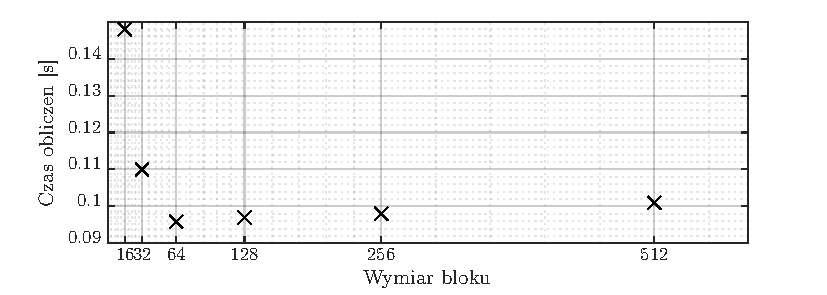
\includegraphics[width=0.8\textwidth]{grafiki/blocksizeplot.pdf}{\caption{Zależność czasu wykonywania programu od wielkości bloku.}}
		\label{fig:blocksize}
\end{figure}

Aby zapobiec konfliktom jednoczesnego odczytywania poprzez kolejne wątki odległych miejsc pamięci karty graficznej, wybrano taką reprezentacje wektorów cząstek, która gwarantuje ciągłość pamięci podczas iterowania po danej współrzędnej wektorów kolejnych cząsteczek. Wymianę danych między pamięcią komputera, a pamięcią karty graficznej ograniczono do niezbędne minimum - w przypadku odczytywania danych z karty do hosta użyto alokacji pamięci typu \textit{pinned}.

Dla każdej z metod przygotowana została odpowiednia klasa zarządzająca cząsteczkami. W kolejnych podsekcjach pokazane zostaną przykładowe kernele wywoływane przez wspomniane  klasy zarządzające.

\subsection{Optymalizacja rojem cząsteczek}
Na listingu \ref{lst:cuda_pso} pokazano kernel odpowiadający za aktualizację pozycji cząsteczki. Najlepsza znana w całym roju pozycja ładowana jest do pamięci \lstinline[style=mycpp]{shared}, ponieważ dane te odczytują wszystkie wątki z danego bloku. Iteratory w petlach \lstinline[style=mycpp]{for} wskazują sposób ułożenia danych w pamięci urządzenia.

\begin{lstlisting}[style=mycpp, label=lst:cuda_pso, caption={Kernel CUDA aktualizujący cząsteczkę PSO.}]
template<int maxDimension>
__global__ void _PsoParticles_updatePositions(float* d_positions, float* d_velocities, float* d_gBestPosition,
	float* d_lBestPositions, curandState* d_prngStates)
{
	int particleId = threadIdx.x + blockIdx.x * blockDim.x;
	if (particleId >= d_particlesNumber)
		return;
	curandState prngLocalState = d_prngStates[particleId];

	__shared__ float gBestPosition[maxDimension];
	for (int i = threadIdx.x; i < d_dimensions; i += blockDim.x)
		gBestPosition[i] = d_gBestPosition[i];
	__syncthreads();

	float randLocal = curand_uniform(&prngLocalState);
	float randGlobal = curand_uniform(&prngLocalState);
	d_prngStates[particleId] = prngLocalState;

	float newVelocity[maxDimension];
	float newPosition[maxDimension];

	float k = 1;
	for (int coordIdx = particleId, i = 0; coordIdx < d_particlesNumber * d_dimensions;
		coordIdx += d_particlesNumber, i++)
	{
		newVelocity[i] = d_psoConstants.w * d_velocities[coordIdx] +
			d_psoConstants.speedLocal * randLocal * (d_lBestPositions[coordIdx] - d_positions[coordIdx]) +
			d_psoConstants.speedGlobal * randGlobal * (gBestPosition[i] - d_positions[coordIdx]);
		newPosition[i] = d_positions[coordIdx] + newVelocity[i];

		// Compute k normalizing coefficient
	}

	for (int coordIdx = particleId, i = 0; coordIdx < d_particlesNumber * d_dimensions;
		coordIdx += d_particlesNumber, i++)
	{
		d_positions[coordIdx] += k * newVelocity[i];
		d_velocities[coordIdx] = k * newVelocity[i];
	}
}
\end{lstlisting}

\subsection{Monte Carlo}
Na listingu \ref{lst:cuda_mc} pokazano kernel odpowiadający za aktualizację pozycji cząsteczki typu Monte Carlo. Kernel losuje przemieszczenie cząsteczki, a następnie normalizuje długość wektora przemieszczenia tak, aby cząsteczka nie wyszła poza dozwolony obszar. Na koniec podejmowana jest decyzja o przemieszczeniu cząsteczki lub też rezygnacji z ruchu.

\begin{lstlisting}[style=mycpp, label=lst:cuda_mc, caption={Kernel CUDA aktualizujący cząsteczkę Monte Carlo.}]
template<int taskId, int maxDimension>
__global__ void _McParticles_McParticles_initialize(float* d_positions, float* d_costs,
	curandState* d_prngStates)
{
	int particleId = threadIdx.x + blockIdx.x * blockDim.x;
	if (particleId >= d_particlesNumber)
		return;
	curandState prngLocalState = d_prngStates[particleId];

	float deltaPosition[maxDimension];
	float newPosition[maxDimension];

	float k = 1;
	for (int coordIdx = particleId, i = 0; coordIdx < d_particlesNumber * d_dimensions;
		coordIdx += d_particlesNumber, i++)
	{
		deltaPosition[i] = (-1 + 2 * curand_uniform(&prngLocalState)) * d_mcConstants.sigma;
		newPosition[i] = d_positions[coordIdx] + deltaPosition[i];

		// Compute k normalizing coefficient
	}
	for (int coordIdx = particleId, i = 0; coordIdx < d_particlesNumber * d_dimensions;
		coordIdx += d_particlesNumber, i++)
		newPosition[i] = d_positions[coordIdx] + k * deltaPosition[i];

	float newCost;
	if(taskId == 1)
		newCost = _PsoParticles_computeCosts_Task1(newPosition);
	else if(taskId == 2)
		newCost = _PsoParticles_computeCosts_Task2(newPosition);

	float currentCost = d_costs[particleId];
	if (newCost < currentCost)
	{
		d_costs[particleId] = newCost;
		for (int coordIdx = particleId, i = 0; coordIdx < d_particlesNumber * d_dimensions;
			coordIdx += d_particlesNumber, i++)
			d_positions[coordIdx] = newPosition[i];
	}
	else
	{
		float rand = curand_uniform(&prngLocalState);
		float threshold = __expf(-(newCost - currentCost) / d_mcConstants.T);
		if (rand < threshold)
		{
			// Save new cost and position analogically
		}
	}
	d_prngStates[particleId] = prngLocalState;
}
\end{lstlisting}

\section{Rozwiązanie zadań dla różnych wymiarów $n$}

Zarówno dla programu implementującego algorytmu PSO i Monte Carlo z wykorzystaniem Open MPI jak i dla programu działającego we współpracy z kartą graficzną przeprowadzono szereg testów optymalizacyjnych dla zadań $1$. oraz $2$ o różnych wymiarach ($n$): $2, \ 10, \ 20, \ 50, \ 100$. Aby~ograniczyć czas wykonywania programów do czasu poniżej $10$ minut, koniczne było w niektórych przypadkach indywidualne dopasowanie parametrów optymalizacji. W ogólności jednak, dla zadań obliczanych metodą PSO użyto następujących parametrów $\omega = \chi$, $c_1 = \chi c_1^*$, $c_2 = \chi c_2^*$, gdzie $\chi = 0.72984$, $c_1^* = c_2^* = 2.05$. W przypadku zadań działających na zasadzie metody Monte Carlo przyjęto ustawienia $\sigma = 0.1$, $T = 0.01$. W większości testów przyjęta warunek stopu akademickiego na poziomie $0.01$.

Sprawdzono działanie programów w optymalizacji problemów o różnej złożoności, tj. każde z zadań zostało rozwiązane dla następujących wymiarów  Aby~ograniczyć działanie programu do czasów wykonywania poniżej $10$ minut, konieczne było w przypadkach o większym wymiarze problemu zwiększenie liczby cząsteczek. Każdy test został wykonany co najmniej $10$ razy, aby móc uśrednić stochastyczny charakter algorytmów. W każdym przypadku położenia początkowe cząsteczek losowano z rozkładu jednostajnego na części obszaru dozwolonego ograniczonego nierównościami kostkowymi $-40 \leq \vect{x}_i \leq -30 \quad i = 1, \ ..., \ n$. Jako kryterium stopu przyjęto kryterium typu akademickiego z warunkiem zakończenia obliczeń $f\left(\vect{x}^{*}\right) < 0.01$.

W kolejnych podrozdziałach opisane zostaną rozwiązania bazujące na technologii MPI (sekcja \ref{sec:table:mpi}) oraz CUDA (sekcja \ref{sec:table:cuda}).

\subsection{Rozwiązanie zadań dla różnych wymiarów $n$ w MPI} \label{sec:table:mpi}

W tabeli \ref{tab:MPI:zad_1} przedstawione zostały pomiary czasu wykonywania programu dla metody PSO oraz Monte Carlo w zadaniu $1$. W przypadku zadania o $n \ = \ 100$ wymiarach konieczne było obniżenie wymagania dot. kryterium stopu do wartości $0.1$. Wyniki pomiarów czasu wykonywania programu dla dla zadania $2$. zebrano w tabeli  \ref{tab:MPI:zad_2}. Dla przypadków o wymiarach $n \ = \ 50$ oraz $n \ = \ 100$ nie udało się znaleźć ustawień optymalizatorów, które pozwoliłyby na rozwiązanie zadań w zadowalającym czasie. Problem ten pojawił się już w poprzedniej części raportu i może wskazywać na naturalne trudności obliczeniowe, które nie są związane z konkretną implementacją.

\renewcommand{\arraystretch}{2}
\begin{table}[H]
\scriptsize
\begin{adjustwidth}{-1.76cm}{}
\centering
\begin{tabular}{|c|c|c|l|l|l|l|l|l|l|l|l|l|}
\hline
\multicolumn{3}{|c|}{Wymiar}                                      & \multicolumn{2}{c|}{2}                             & \multicolumn{2}{c|}{10}                            & \multicolumn{2}{c|}{20}                            & \multicolumn{2}{c|}{50}                            & \multicolumn{2}{c|}{100}                           \\ \hline
\multicolumn{3}{|c|}{Algorytm}                                    & \multicolumn{1}{c|}{PSO} & \multicolumn{1}{c|}{MC} & \multicolumn{1}{c|}{PSO} & \multicolumn{1}{c|}{MC} & \multicolumn{1}{c|}{PSO} & \multicolumn{1}{c|}{MC} & \multicolumn{1}{c|}{PSO} & \multicolumn{1}{c|}{MC} & \multicolumn{1}{c|}{PSO} & \multicolumn{1}{c|}{MC} \\ \hline
\multicolumn{3}{|c|}{Liczba cząsteczek}                           & $10^{2}$                 & $10^{2}$                & $10^{2}$                 & $10^{2}$                & $10^{3}$                 & $10^{3}$                & $10^{3}$                 & $10^{3}$                & $10^{3}$                 & $10^{3}$                \\ \hline
\multirow{8}{*}{Czas} & \multirow{4}{*}{Sekwencyjnie} & Średnia   & $7.7 \ 10^{-2}$          & $6.6 \ 10^{-3}$         & $9.9 \ 10^{-2}$          & $2.5 \ 10^{-1}$         & $7.4 \ 10^{-1}$          & $6.6 \ 10^{0}$          & $5.6 \ 10^{0}$           & $4.3 \ 10^{1}$          & $8.5 \ 10^{1}$           & $7.9 \ 10^{1}$          \\ \cline{3-13} 
                      &                               & Minimum   & $3.0 \ 10^{-2}$          & $3.2 \ 10^{-3}$         & $6.3 \ 10^{-2}$          & $2.1 \ 10^{-1}$         & $4.8 \ 10^{-1}$          & $6.0 \ 10^{0}$          & $3.9 \ 10^{0}$           & $3.6 \ 10^{1}$          & $3.3 \ 10^{1}$           & $7.8 \ 10^{1}$          \\ \cline{3-13} 
                      &                               & Maksimum  & $2.0 \ 10^{-1}$          & $1.2 \ 10^{-2}$         & $1.6 \ 10^{-1}$          & $2.8  \ 10^{-1}$        & $8.9 \ 10^{-1}$          & $7.4 \ 10^{0}$          & $5.4 \ 10^{0}$           & $4.9 \ 10^{1}$          & $1.3 \ 10^{1}$           & $8.0 \ 10^{1}$          \\ \cline{3-13} 
                      &                               & Wariancja & $1.7 \ 10^{-3}$          & $7.9 \ 10^{-6}$         & $7.5 \ 10^{-4}$          & $3.3 \ 10^{-4}$         & $8.9 \ 10^{-3}$          & $1.4 \ 10^{-1}$         & $1.8 \ 10^{-1}$          & $1.8 \ 10^{1}$          & $5.9 \ 10^{2}$           & $8.9 \ 10^{-1}$         \\ \cline{2-13} 
                      & \multirow{4}{*}{Równolegle}   & Średnia   & $4.7 \ 10^{-2}$          & $1.2 \ 10^{-3}$         & $4.9 \ 10^{-1}$          & $4.9 \ 10^{-2}$         & $3.5 \ 10^{-1}$          & $1.2 \ 10^{0}$          & $3.6 \ 10^{0}$           & $8.0 \ 10^{0}$          & $5.1 \ 10^{1}$           & $1.4 \ 10^{1}$          \\ \cline{3-13} 
                      &                               & Minimum   & $1.8 \ 10^{-3}$          & $5.3 \ 10^{-5}$         & $7.4 \ 10^{-2}$          & $3.7 \ 10^{-2}$         & $2.3 \ 10^{-1}$          & $1.0 \ 10^{0}$          & $2.6 \ 10^{0}$           & $6.1 \ 10^{0}$          & $3.3 \ 10^{1}$           & $1.3 \ 10^{1}$          \\ \cline{3-13} 
                      &                               & Maksimum  & $2.5 \ 10^{0}$           & $5.5 \ 10^{-3}$         & $2.2 \ 10^{0}$           & $5.7 \ 10^{-2}$         & $7.0 \ 10^{-1}$          & $1.3 \ 10^{0}$          & $5.6 \ 10^{0}$           & $1.3 \ 10^{1}$          & $7.0 \ 10^{1}$           & $1.4 \ 10^{1}$          \\ \cline{3-13} 
                      &                               & Wariancja & $1.7 \ 10^{-1}$          & $8.7 \ 10^{-7}$         & $2.3 \ 10^{-1}$          & $2.2 \ 10^{-5}$         & $8 \ 10^{-3}$            & $4.1 \ 10^{-3}$         & $4.1 \ 10^{-1}$          & $3.5 \ 10^{0}$          & $1.2 \ 10^{2}$           & $7.9 \ 10^{-2}$         \\ \hline
\end{tabular}
\end{adjustwidth}
\caption{Rozwiązania zadania $1$. dla różnych wymiarów $n$ i ustawień (OpenMPI).}
\label{tab:MPI:zad_1}
\end{table}

\renewcommand{\arraystretch}{2}
\begin{table}[H]
\scriptsize
\begin{adjustwidth}{-1.76cm}{}
\centering
\begin{tabular}{|c|c|c|l|l|l|l|l|l|c|c|c|c|}
\hline
\multicolumn{3}{|c|}{Wymiar}                                      & \multicolumn{2}{c|}{2}                             & \multicolumn{2}{c|}{10}                            & \multicolumn{2}{c|}{20}                            & \multicolumn{2}{c|}{50} & \multicolumn{2}{c|}{100} \\ \hline
\multicolumn{3}{|c|}{Algorytm}                                    & \multicolumn{1}{c|}{PSO} & \multicolumn{1}{c|}{MC} & \multicolumn{1}{c|}{PSO} & \multicolumn{1}{c|}{MC} & \multicolumn{1}{c|}{PSO} & \multicolumn{1}{c|}{MC} & PSO         & MC        & PSO         & MC         \\ \hline
\multicolumn{3}{|c|}{Liczba cząsteczek}                           & $10^{2}$                 & $10^{2}$                & $10^{2}$                 & $10^{2}$                & $10^{4}$                 & $10^{4}$                & -           & -         & -           & -          \\ \hline
\multirow{8}{*}{Czas} & \multirow{4}{*}{Sekwencyjnie} & Średnia   & $4.3 \ 10^{-2}$          & $1.1 \ 10^{-1}$         & $3.8 \ 10^{-1}$          & $8.1 \ 10^{0}$          & $6.6 \ 10^{0}$           & $8.6 \ 10^{0}$          & -           & -         & -           & -          \\ \cline{3-13} 
                      &                               & Minimum   & $2.3 \ 10^{-2}$          & $4.7 \ 10^{-2}$         & $2.2 \ 10^{-1}$          & $1.1 \ 10^{0}$          & $5.3 \ 10^{0}$           & $6.0 \ 10^{0}$          & -           & -         & -           & -          \\ \cline{3-13} 
                      &                               & Maksimum  & $8.6 \ 10^{-2}$          & $2.2 \ 10^{-1}$         & $6.4 \ 10^{-1}$          & $1.6 \ 10^{0}$          & $9.7 \ 10^{0}$           & $1.2 \ 10^{1}$          & -           & -         & -           & -          \\ \cline{3-13} 
                      &                               & Wariancja & $4.7 \ 10^{-4}$          & $1.9 \ 10^{-3}$         & $1.3 \ 10^{-3}$          & $1.9 \ 10^{-1}$         & $1.1 \ 10^{0}$           & $3.4 \ 10^{-1}$         & -           & -         & -           & -          \\ \cline{2-13} 
                      & \multirow{4}{*}{Równolegle}   & Średnia   & $2.7 \ 10^{-2}$          & $3.3 \ 10^{-2}$         & $1.4 \ 10^{-1}$          & $1.4 \ 10^{0}$          & $1.3 \ 10^{0}$           & $1.5 \ 10^{0}$          & -           & -         & -           & -          \\ \cline{3-13} 
                      &                               & Minimum   & $3.5 \ 10^{-3}$          & $4.4 \ 10^{-3}$         & $2.8 \ 10^{-1}$          & $1.1 \ 10^{0}$          & $7.7 \ 10^{-1}$          & $9.0 \ 10^{-1}$         & -           & -         & -           & -          \\ \cline{3-13} 
                      &                               & Maksimum  & $2.9 \ 10^{-1}$          & $5.9 \ 10^{-2}$         & $8.4 \ 10^{-2}$          & $1.6 \ 10^{0}$          & $3.1 \ 10^{0}$           & $1.8 \ 10^{0}$          & -           & -         & -           & -          \\ \cline{3-13} 
                      &                               & Wariancja & $2.7 \ 10^{-3}$          & $2.8 \ 10^{-4}$         & $1.4 \ 10^{-3}$          & $1.9 \ 10^{-2}$         & $2.3 \ 10^{-2}$          & $1.1 \ 10^{-1}$         & -           & -         & -           & -          \\ \hline
\end{tabular}
\end{adjustwidth}
\caption{Rozwiązania zadania $2$. dla różnych wymiarów $n$ i ustawień (OpenMPI).}
\label{tab:MPI:zad_2}
\end{table}

Na rys. \ref{fig:przysp:zad1}. i \ref{fig:przysp:zad2} pokazano przyspieszenia implementacji równoległej PSO i Monte Carlo z wykorzystaniem MPI. 

\begin{figure}[H]
\centering
\begin{minipage}[b]{\dimexpr.5\textwidth-1em}
  \centering
  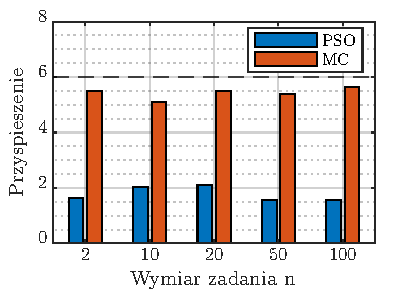
\includegraphics[width=1\linewidth]{grafiki/przyspieszenieMPI1.pdf}
  \captionof{figure}{Średnie przyspieszenie implementacji równoległej podczas prób optymalizacji zad. $1$.}
  \label{fig:przysp:zad1}
\end{minipage} \hfill
\begin{minipage}[b]{\dimexpr.5\textwidth-1em}
  \centering
  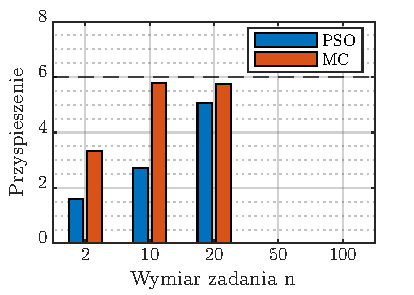
\includegraphics[width=1\linewidth]{grafiki/przyspieszenieMPI2.pdf}
  \captionof{figure}{Średnie przyspieszenie implementacji równoległej podczas prób optymalizacji zad. $2$.}
  \label{fig:przysp:zad2}
\end{minipage}
\end{figure}

\subsection{Rozwiązanie zadań dla różnych wymiarów $n$ w CUDA} \label{sec:table:cuda}
W tabeli \ref{tab:CUDA} przedstawione zostały pomiary czasu wykonywania zadań $1$. i $2$. dla metody PSO oraz~Monte Carlo. W przypadku zadania o $n \ = \ 100$ wymiarach konieczne było obniżenie wymagania dot. kryterium stopu do wartości $0.1$. Podobnie jak w poprzednich badaniach, nie udało rozwiązać się wysokowymiarowych zadań optymalizacji funkcji Rosenbrocka.

Wykorzystanie karty graficznej i sposób implementacji algorytmu pozwala na znaczne zwiększenie liczby symulowanych cząsteczek. Dzięki temu udało się rozwiązać testowy przypadek z zadania optymalizacji $1.$ dla $n \ = \ 200$ wymiarów. Do obliczeń wykorzystano rój o wielkości $1 \ 000 \ 000$ cząsteczek, a średni czas obliczeń dla takiego zestawu parametrów wyniósł $7.3 \ s$. Taka liczba cząsteczek byłaby niemożliwa do obsłużenia w rozsądnym czasie w implementacji na CPU.

Możemy także porównać czasy działania programu z akceleracją GPU i innych wersji równoległych - na maszyny z pamięcią globalną oraz lokalną. Widoczne jest, że GPU sprawdza się w zadaniach z~dużą liczbą cząsteczek - dużą ilością danych do przetworzenia. Dla zadań o małej liczbie cząstek i~wymiarów zysk jest znikomy lub wersje programów na GPU działają gorzej niż ich odpowiedniki przeznaczone do obliczeń na CPU. Duża liczba cząsteczek pozwala lepiej ukryć opóźnienia w dostępie do pamięci na karcie graficznej i~zniwelować niską przepustowość magistrali.

Mogłoby się wydawać, że skoro dostępna jest moc obliczeniowa karty graficznej i w konsekwencji przetwarzanie wektorowe, to najlepszą strategią optymalizacji z cząsteczkami jest użycie ich jak największej liczby. Pośrednie wyniki uzyskane podczas testów wskazywały, że może istnieć optymalna liczba lub zagęszczenie cząsteczek, powyżej której zbieżność algorytmów znacznie spada. Efekt ten widoczny był szczególnie w przypadku PSO, które powyżej pewnego zagęszczenia cząsteczek nie dawało lepszych rezultatów.

\renewcommand{\arraystretch}{2}
\begin{table}[H]
\scriptsize
\begin{adjustwidth}{-1.76cm}{}
\centering
\begin{tabular}{|c|c|c|l|l|l|l|l|l|c|c|c|c|}
\hline
\multicolumn{3}{|c|}{Wymiar}                                   & \multicolumn{2}{c|}{2}                             & \multicolumn{2}{c|}{10}                            & \multicolumn{2}{c|}{20}                            & \multicolumn{2}{c|}{50}                                                         & \multicolumn{2}{c|}{100}                                                        \\ \hline
\multicolumn{3}{|c|}{Algorytm}                                 & \multicolumn{1}{c|}{PSO} & \multicolumn{1}{c|}{MC} & \multicolumn{1}{c|}{PSO} & \multicolumn{1}{c|}{MC} & \multicolumn{1}{c|}{PSO} & \multicolumn{1}{c|}{MC} & PSO                                    & MC                                     & PSO                                    & MC                                     \\ \hline
\multicolumn{3}{|c|}{\textbf{Liczba cząsteczek}}               & \textbf{$10^{2}$}        & \textbf{$10^{2}$}       & \textbf{$10^{2}$}        & \textbf{$10^{2}$}       & \textbf{$10^{3}$}        & \textbf{$10^{3}$}       & \multicolumn{1}{l|}{\textbf{$10^{3}$}} & \multicolumn{1}{l|}{\textbf{$10^{3}$}} & \multicolumn{1}{l|}{\textbf{$10^{3}$}} & \multicolumn{1}{l|}{\textbf{$10^{3}$}} \\ \hline
\multirow{4}{*}{Czas} & \multirow{4}{*}{Zad. $1$.} & Średnia   & $3.5 \ 10^{-3}$          & $2.8 \ 10^{-2}$         & $7.6 \ 10^{-2}$          & $5.4 \ 10^{-1}$         & $1.2 \ 10^{-2}$          & $8.4 \ 10^{-1}$         & \multicolumn{1}{l|}{$3.6 \ 10^{-2}$}   & \multicolumn{1}{l|}{$3.3 \ 10^{0}$}    & \multicolumn{1}{l|}{$8.6 \ 10^{-1}$}   & \multicolumn{1}{l|}{$3.2 \ 10^{0}$}    \\ \cline{3-13} 
                      &                            & Minimum   & $1.4 \ 10^{-3}$          & $1.3 \ 10^{-2}$         & $3.8 \ 10^{-3}$          & $4.2 \ 10^{-1}$         & $7.7 \ 10^{-3}$          & $7.3 \ 10^{-1}$         & \multicolumn{1}{l|}{$2.9 \ 10^{-2}$}   & \multicolumn{1}{l|}{$2.3 \ 10^{0}$}    & \multicolumn{1}{l|}{$4.7 \ 10^{-1}$}   & \multicolumn{1}{l|}{$3.1 \ 10^{0}$}    \\ \cline{3-13} 
                      &                            & Maksimum  & $5.6 \ 10^{-3}$          & $3.7 \ 10^{-2}$         & $1.4 \ 10^{0}$           & $6.2 \ 10^{-1}$         & $1.8 \ 10^{-2}$          & $9.2 \ 10^{-1}$         & \multicolumn{1}{l|}{$4.6 \ 10^{-2}$}   & \multicolumn{1}{l|}{$4.9 \ 10^{0}$}    & \multicolumn{1}{l|}{$1.2 \ 10^{0}$}    & \multicolumn{1}{l|}{$3.3 \ 10^{0}$}    \\ \cline{3-13} 
                      &                            & Wariancja & $1.5 \ 10^{-6}$          & $6.6 \ 10^{-5}$         & $9.0 \ 10^{-2}$          & $4.6 \ 10^{-3}$         & $5.5 \ 10^{-6}$          & $4.8 \ 10^{-3}$         & \multicolumn{1}{l|}{$2.8 \ 10^{-5}$}   & \multicolumn{1}{l|}{$8.0 \ 10^{-1}$}   & \multicolumn{1}{l|}{$6.56 \ 10^{-2}$}  & \multicolumn{1}{l|}{$5.6 \ 10^{0}$}    \\ \hline
\multicolumn{3}{|c|}{\textbf{Liczba cząsteczek}}               & \textbf{$10^{2}$}        & \textbf{$10^{2}$}       & \textbf{$10^{2}$}        & \textbf{$10^{2}$}       & \textbf{$10^{4}$}        & \textbf{$10^{4}$}       & \textbf{-}                             & \textbf{-}                             & \textbf{-}                             & \textbf{-}                             \\ \hline
\multirow{4}{*}{Czas} & Zad. $2$.                  & Średnia   & $1.2 \ 10^{-2}$          & $1.2 \ 10^{0}$          & $3.5 \ 10^{0}$           & $7.2 \ 10^{0}$          & $8.9 \ 10^{-1}$          & $1.8 \ 10^{0}$          & \textbf{-}                             & \textbf{-}                             & \textbf{-}                             & \textbf{-}                             \\ \cline{3-13} 
                      &                            & Minimum   & $4.9 \ 10^{-3}$          & $2.3 \ 10^{-2}$         & $1.8 \ 10^{0}$           & $6.1 \ 10^{0}$          & $1.9 \ 10^{-1}$          & $1.5 \ 10^{0}$          & \textbf{-}                             & \textbf{-}                             & \textbf{-}                             & \textbf{-}                             \\ \cline{3-13} 
                      &                            & Maksimum  & $2.4 \ 10^{-2}$          & $3.3 \ 10^{0}$          & $7.4 \ 10^{0}$           & $7.8 \ 10^{0}$          & $3.7 \ 10^{0}$           & $2.4 \ 10^{0}$          & \textbf{-}                             & \textbf{-}                             & \textbf{-}                             & \textbf{-}                             \\ \cline{3-13} 
                      &                            & Wariancja & $3.9 \ 10^{-5}$          & $2.3 \ 10^{0}$          & $2.8 \ 10^{0}$           & $3.7 \ 10^{-1}$         & $1.1 \ 10^{0}$           & $1.1 \ 10^{-1}$         & \textbf{-}                             & \textbf{-}                             & \textbf{-}                             & \textbf{-}                             \\ \hline
\end{tabular}
\end{adjustwidth}
\caption{Rozwiązania zadania $1$. i $2$. dla różnych wymiarów $n$ i ustawień (CUDA).}
\label{tab:CUDA}
\end{table}

\section{Porównanie trajektorii dla $n = 2$}

W tej części sprawozdania przedstawiono wyniki uzyskane dla cząsteczki dwuwymiarowej dla obu zadań i dla obu algorytmów. W pierwszej części (\ref{sec:MPI2}) pokazano wyniki otrzymane dla MPI, a w drugiej  (\ref{sec:CUDA2})-- dla CUDA.

\subsection{Porównanie trajektorii dla $n = 2$ w MPI} \label{sec:MPI2}

Na wykresach \ref{fig:koszt:PSO1} - \ref{fig:koszt:MC2} zostało pokazane jak zmienia się koszt w kolejnych iteracjach dla najlepszych położeń. Z wykresów tych widać, że wartość kosztu osiąga okolice 0 po podobnej liczbie iteracji dla obu algorytmów. Różnica jest minimalna w przypadku zadania 1 -- na rzecz algorytmu PSO, a w przypadku zadania 2 -- na rzecz algorytmu Monte Carlo.

%Funkcja kosztu - zad1 i zad2 dla najlepszej cząsteczki
\begin{figure}[H]
\centering
\begin{minipage}[b]{\dimexpr.5\textwidth-1em}
  \centering
  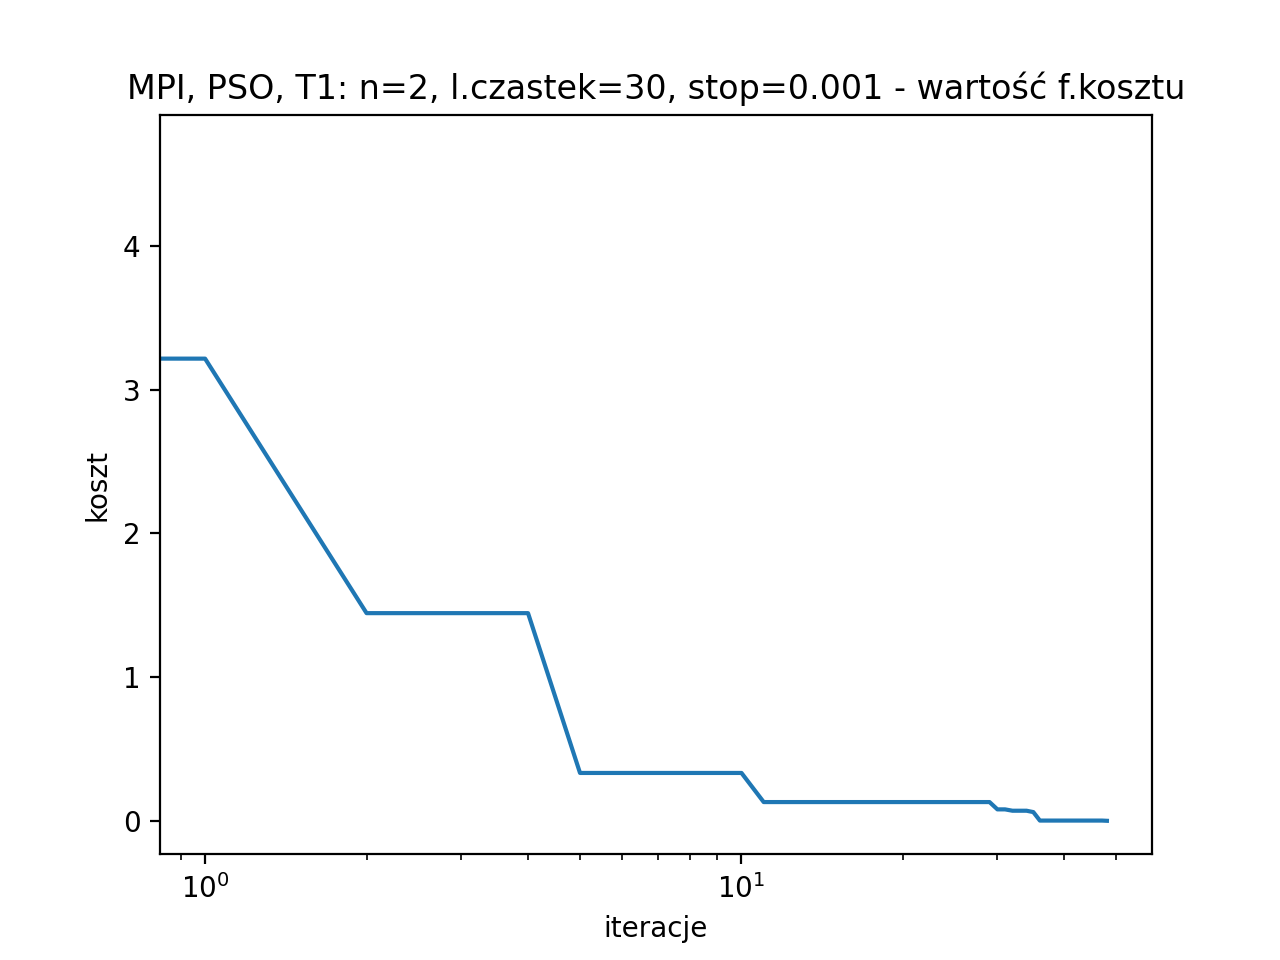
\includegraphics[width=1\linewidth]{grafiki/MPI_PSO_T1/MPI_PSO_T1_koszt_monotoniczny.png}
  \captionof{figure}{Wartość funkcji kosztu dla zadania $1$ dla metody PSO.}
  \label{fig:koszt:PSO1}
\end{minipage} \hfill
\begin{minipage}[b]{\dimexpr.5\textwidth-1em}
  \centering
  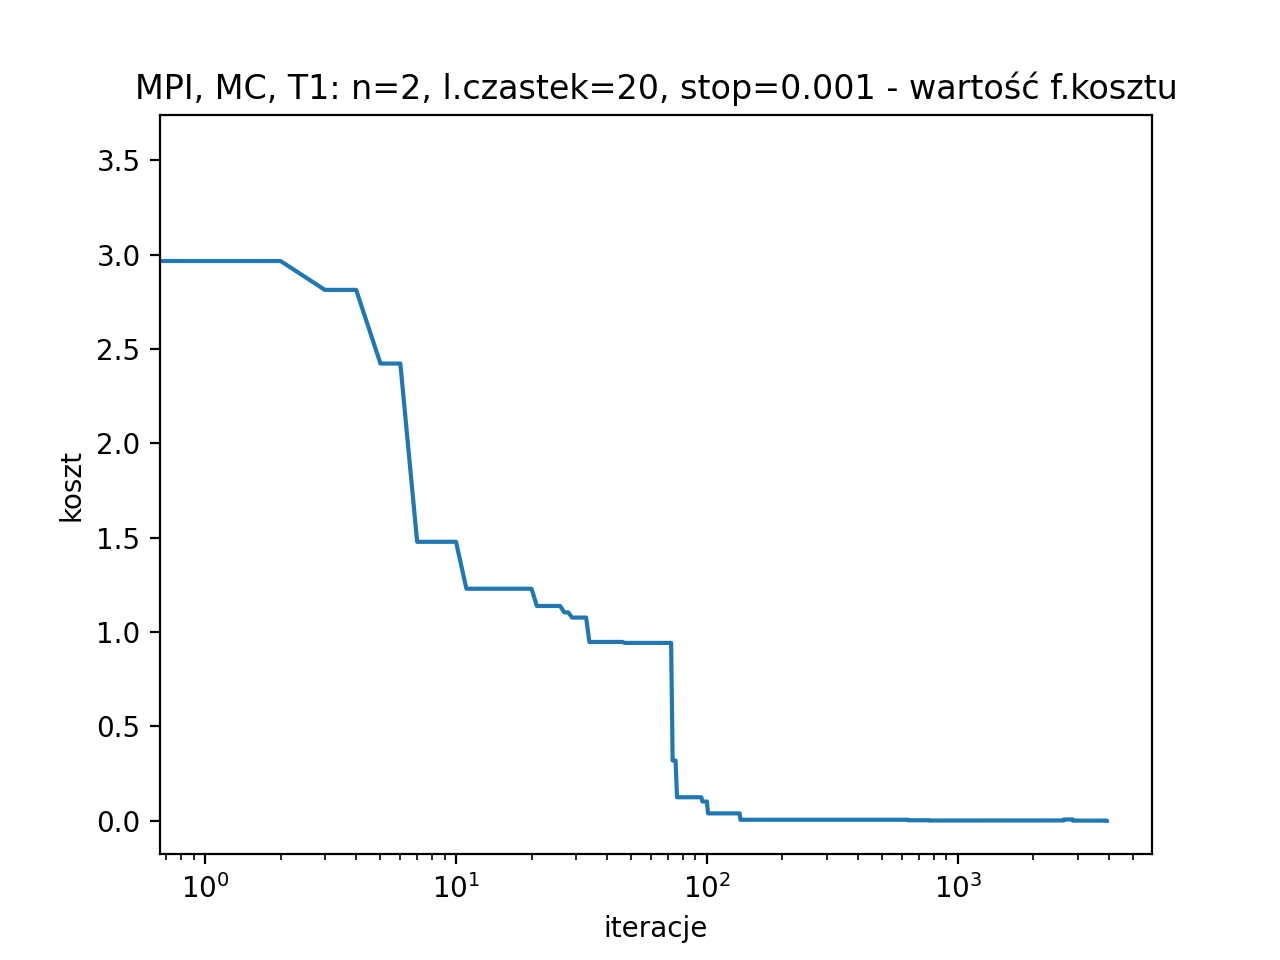
\includegraphics[width=1\linewidth]{grafiki/MPI_MC_T1/MPI_MC_T1_koszt.png}
  \captionof{figure}{Wartość funkcji kosztu dla zadania $1$ dla metody Monte Carlo.}
  \label{fig:koszt:MC1}
\end{minipage}
\end{figure}

\begin{figure}[H]
\centering
\begin{minipage}[b]{\dimexpr.5\textwidth-1em}
  \centering
  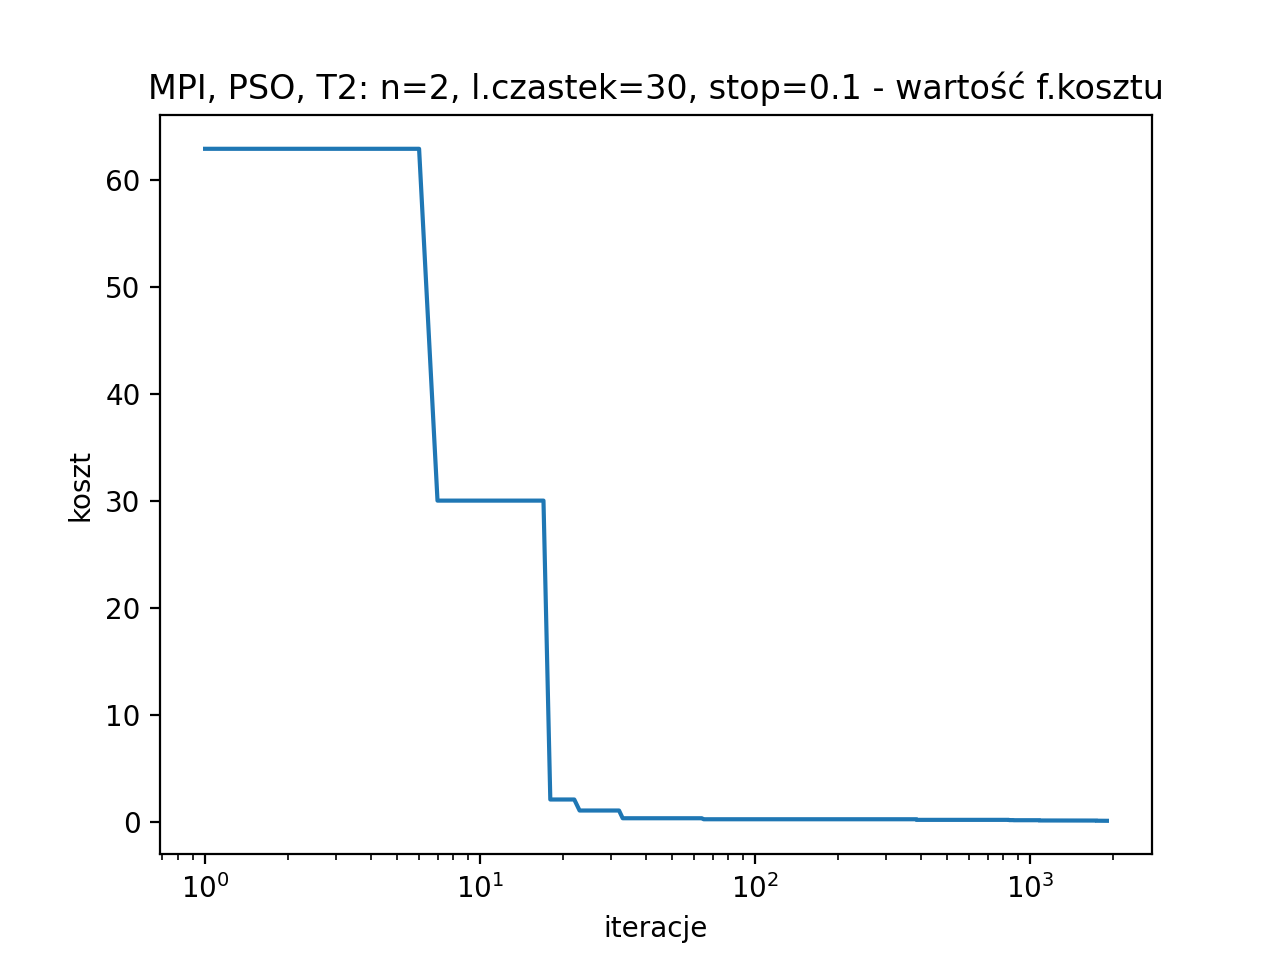
\includegraphics[width=1\linewidth]{grafiki/MPI_PSO_T2/MPI_PSO_T2_koszt_monotoniczny.png}
  \captionof{figure}{Wartość funkcji kosztu dla zadania $2$ dla metody PSO.}
  \label{fig:koszt:PSO2}
\end{minipage} \hfill
\begin{minipage}[b]{\dimexpr.5\textwidth-1em}
  \centering
  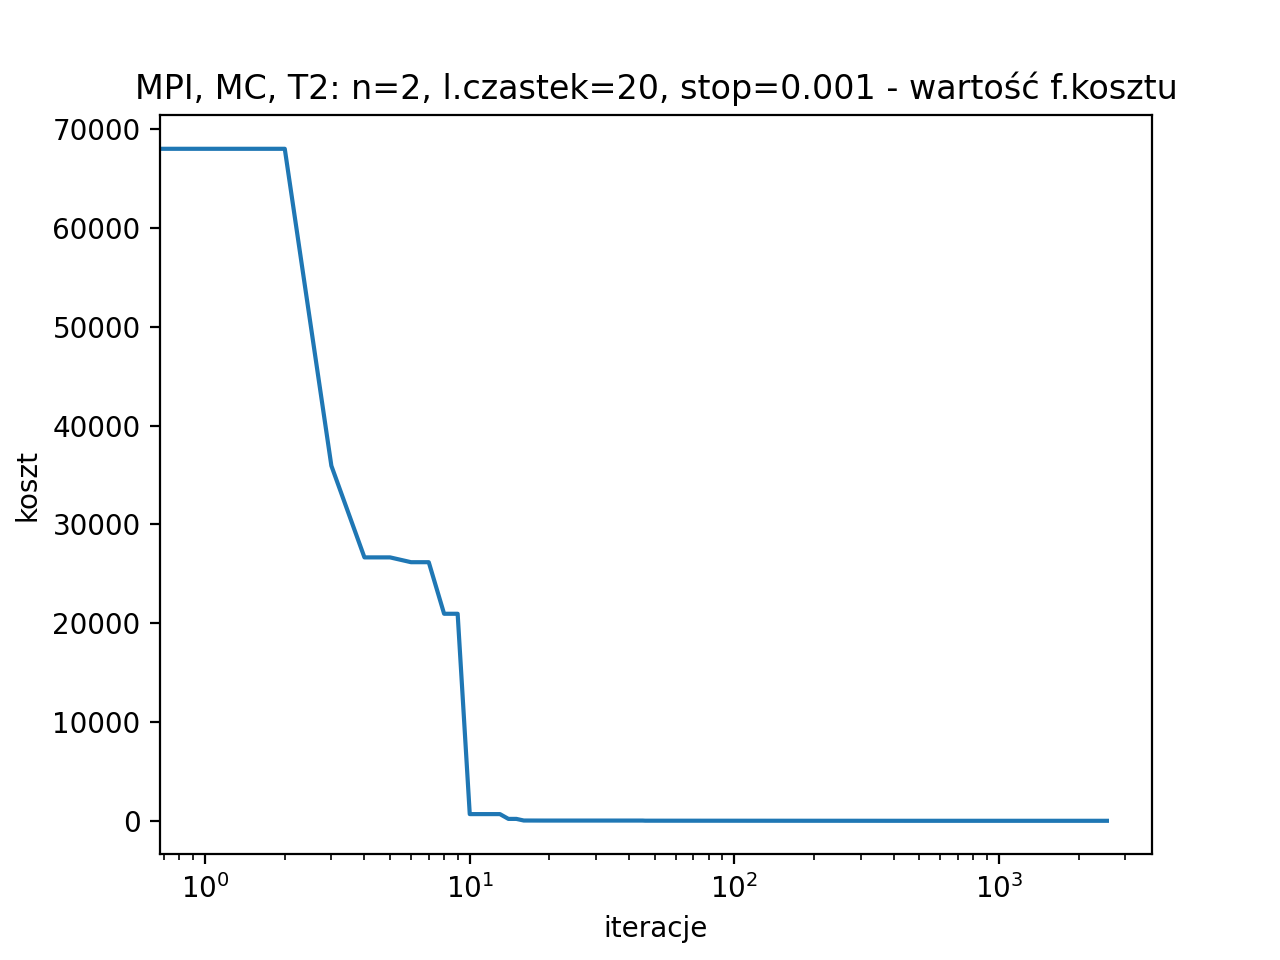
\includegraphics[width=1\linewidth]{grafiki/MPI_MC_T2/MPI_MC_T2_koszt.png}
  \captionof{figure}{Wartość funkcji kosztu dla zadania $2$ dla metody Monte Carlo.}
  \label{fig:koszt:MC2}
\end{minipage}
\end{figure}

Na kolejnych wykresach \ref{fig:pozycjeStartowe:PSO1} - \ref{fig:pozycjeStartowe:MC2} przedstawiono pozycje startowe przykładowych cząsteczek, a na kolejnych wykresach   \ref{fig:pozycjeStartowe:PSO1} - \ref{fig:pozycjeStartowe:MC2} trajektorię ruchu przykładowych cząsteczek. Widać, ze dzięki zmodyfikowaniu algorytmu Monte Carlo cząsteczka dąży prosto do celu, czyli do jak najmniejszego kosztu. To może powodować wpadnięcie w lokalne minimum bez możliwości wyjścia z niego, choc podjęta przez nas modyfikacja może czasem temu zapobiec. Natomiast losowanie odpowiednio dużej liczby cząsteczek powoduje, ze znajdowana jest taka, która ląduje w minimum globalnym. Natomiast dla algorytmu PSO widać, że cząsteczki potrafią wyjść poza lokalne minima i dlatego ich trajektoria jest mniej prosta.


%Pozycje startowe
\begin{figure}[H]
\centering
\begin{minipage}[b]{\dimexpr.5\textwidth-1em}
  \centering
  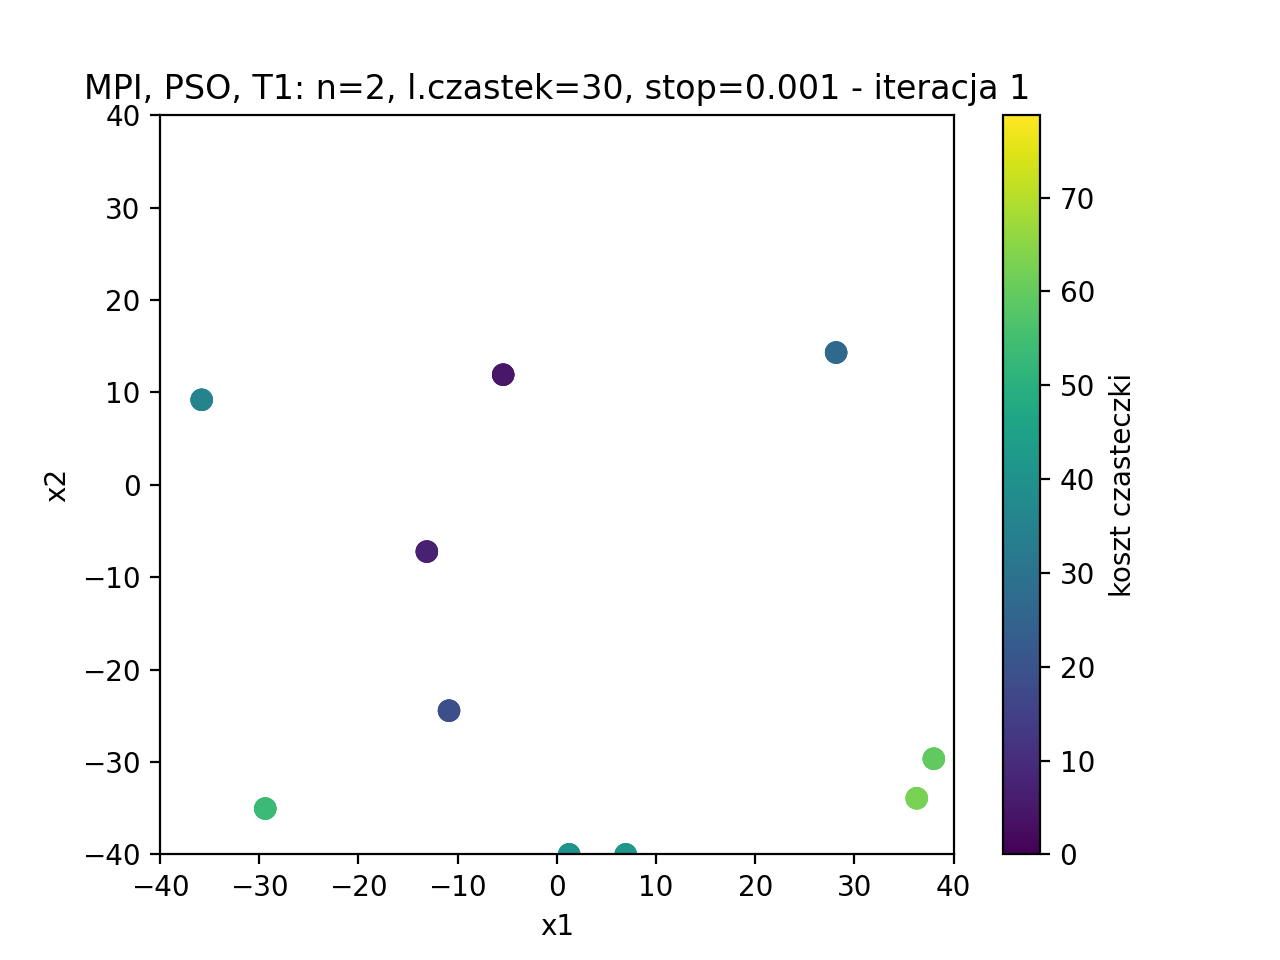
\includegraphics[width=1\linewidth]{grafiki/MPI_PSO_T1/MPI_PSO_T1_startPositions.png}
  \captionof{figure}{Pozycje startowe cząsteczek dla algorytmu PSO dla zadania $1$.}
  \label{fig:pozycjeStartowe:PSO1}
\end{minipage} \hfill
\begin{minipage}[b]{\dimexpr.5\textwidth-1em}
  \centering
  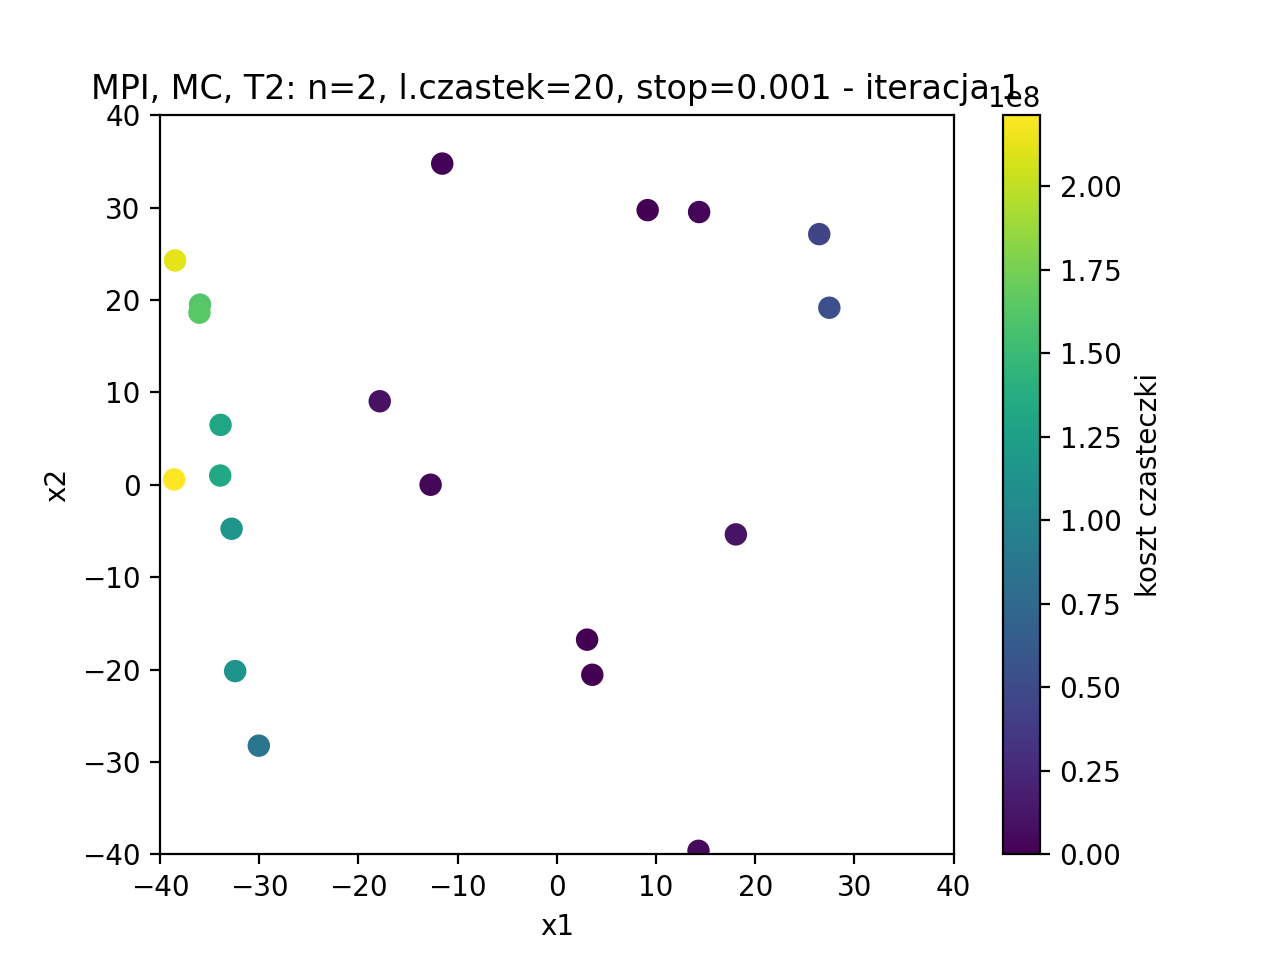
\includegraphics[width=1\linewidth]{grafiki/MPI_MC_T2/MPI_MC_T2_startPositions.png}
  \captionof{figure}{Pozycje startowe cząsteczek dla algorytmu MC dla zadania $1$.}
  \label{fig:pozycjeStartowe:MC1}
\end{minipage}
\end{figure}

\begin{figure}[H]
\centering
\begin{minipage}[b]{\dimexpr.5\textwidth-1em}
  \centering
  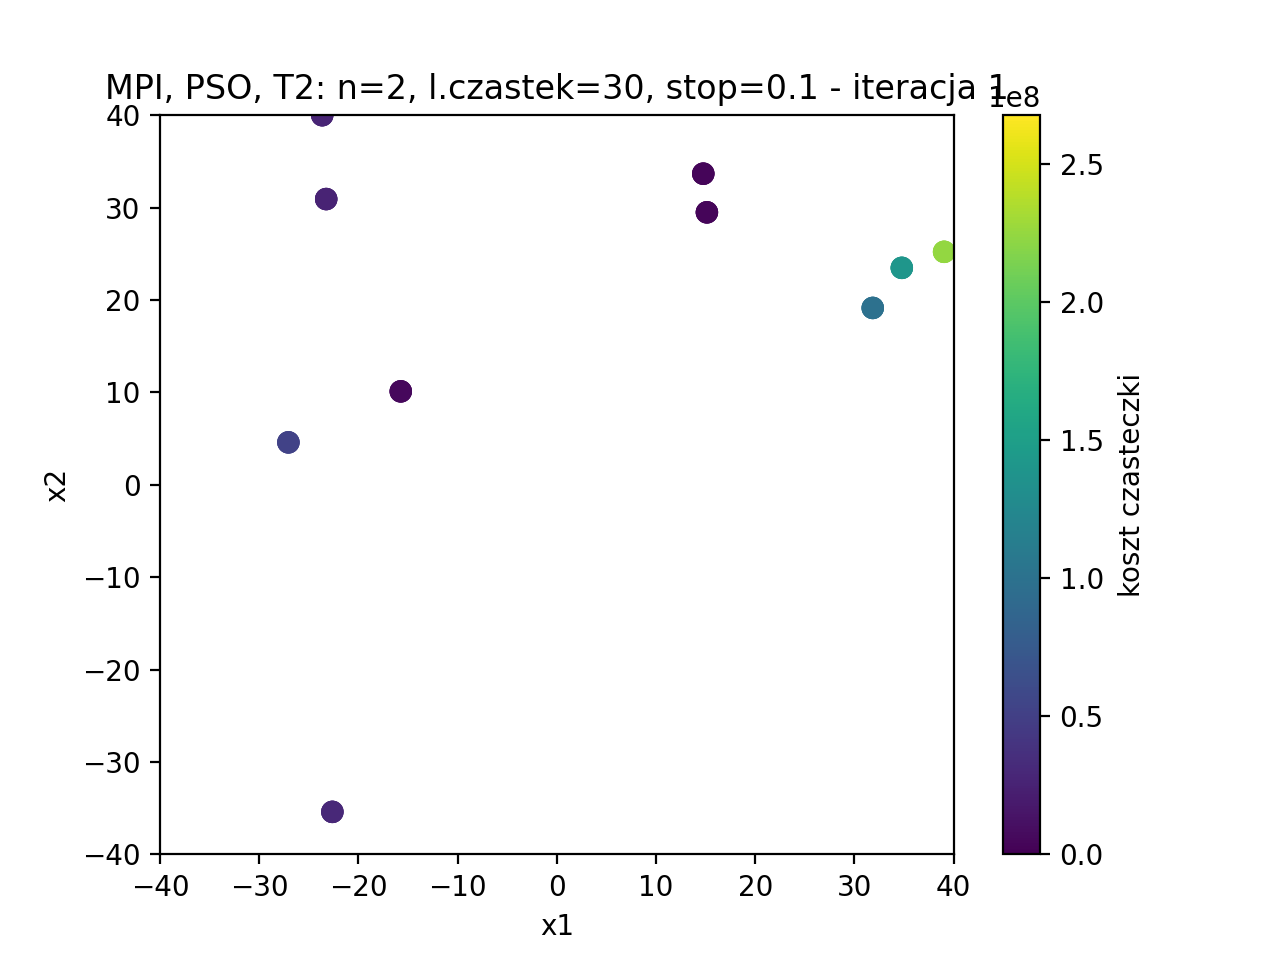
\includegraphics[width=1\linewidth]{grafiki/MPI_PSO_T2/MPI_PSO_T2_startPositions.png}
  \captionof{figure}{Pozycje startowe cząsteczek dla algorytmu PSO dla zadania $2$.}
  \label{fig:pozycjeStartowe:PSO2}
\end{minipage} \hfill
\begin{minipage}[b]{\dimexpr.5\textwidth-1em}
  \centering
  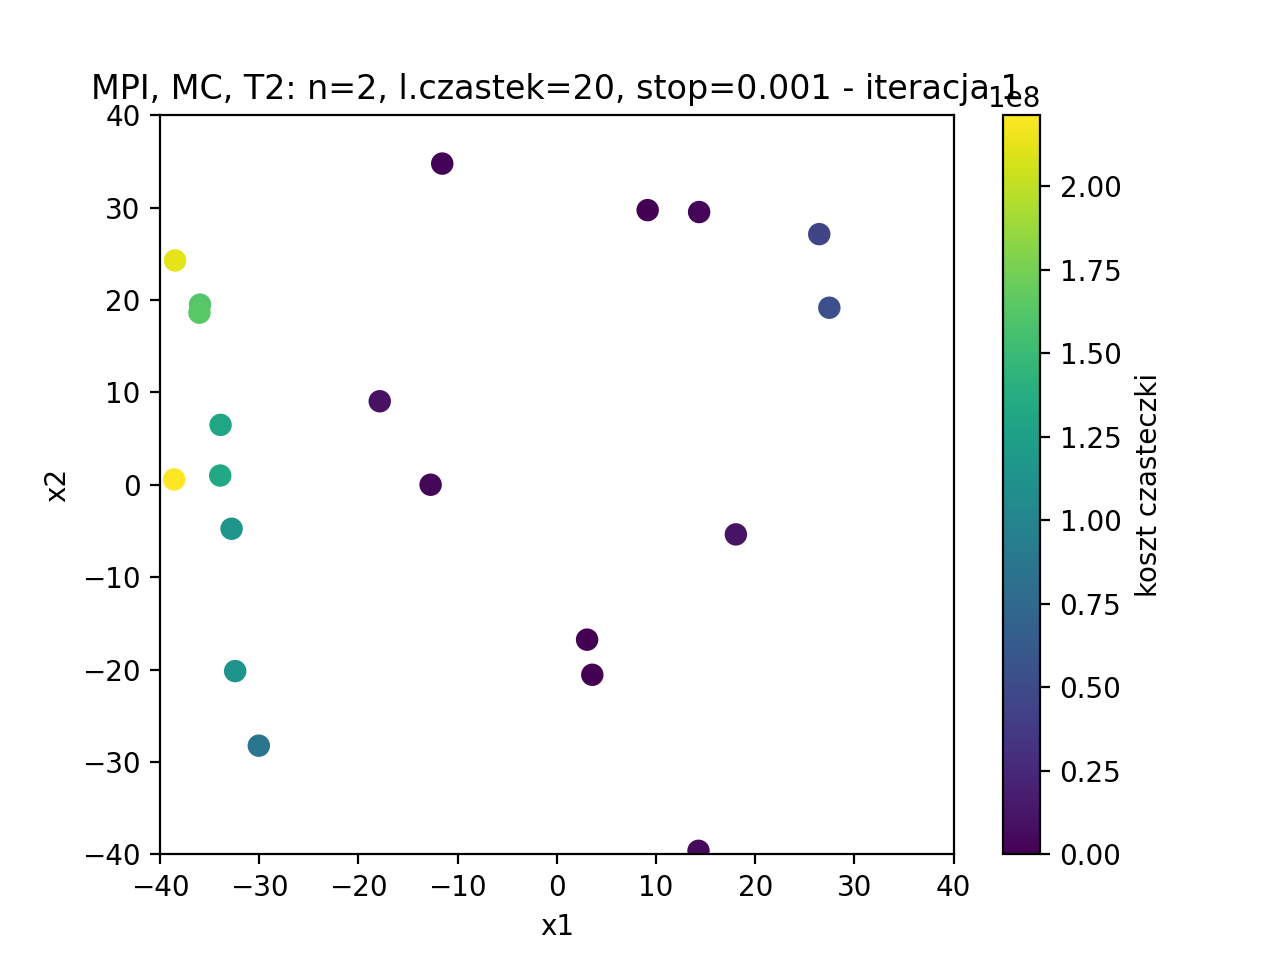
\includegraphics[width=1\linewidth]{grafiki/MPI_MC_T2/MPI_MC_T2_startPositions.png}
  \captionof{figure}{Pozycje startowe cząsteczek dla algorytmu MC dla zadania $2$.}
  \label{fig:pozycjeStartowe:MC2}
\end{minipage}
\end{figure}

% Trajektoria wybranej cząstki

\begin{figure}[H]
\centering
\begin{minipage}[b]{\dimexpr.5\textwidth-1em}
  \centering
  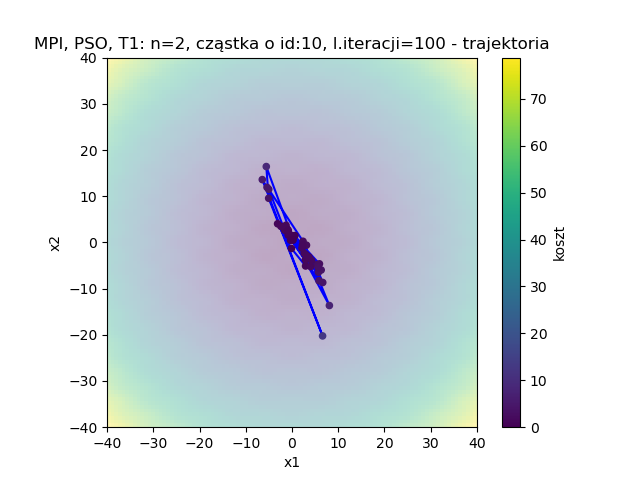
\includegraphics[width=1\linewidth]{grafiki/MPI_PSO_T1/MPI_PSO_T1_trajectory_id10.png}
  \captionof{figure}{Trajektoria wybranej cząstki dla algorytmu PSO dla zadania $1$.}
  \label{fig:trajektoriaWybrana:PSO1}
\end{minipage} \hfill
\begin{minipage}[b]{\dimexpr.5\textwidth-1em}
  \centering
  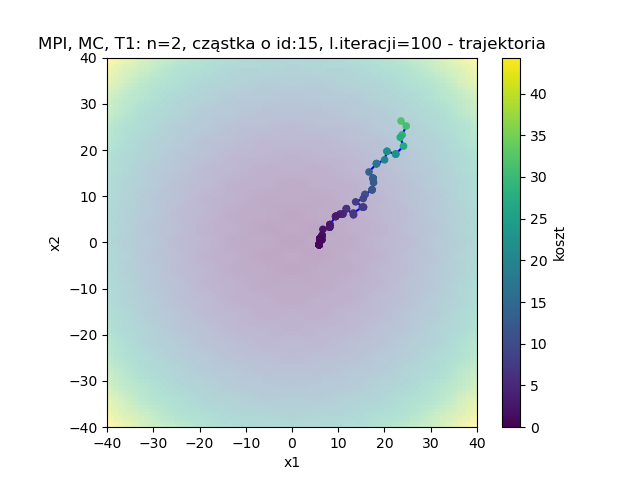
\includegraphics[width=1\linewidth]{grafiki/MPI_MC_T1/MPI_ MC_T1_trajectory_id15.png}
  \captionof{figure}{Trajektoria wybranej cząstki dla algorytmu MC dla zadania $1$.}
  \label{fig:trajektoriaWybrana:MC1}
\end{minipage}
\end{figure}

\begin{figure}[H]
\centering
\begin{minipage}[b]{\dimexpr.5\textwidth-1em}
  \centering
  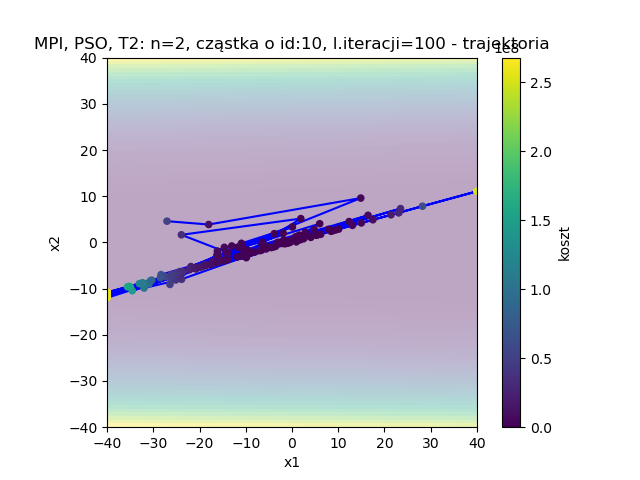
\includegraphics[width=1\linewidth]{grafiki/MPI_PSO_T2/MPI_ PSO_T2_trajectory_id10.png}
  \captionof{figure}{Trajektoria wybranej cząstki dla algorytmu PSO dla zadania $2$.}
  \label{fig:trajektoriaWybrana:PSO2}
\end{minipage} \hfill
\begin{minipage}[b]{\dimexpr.5\textwidth-1em}
  \centering
  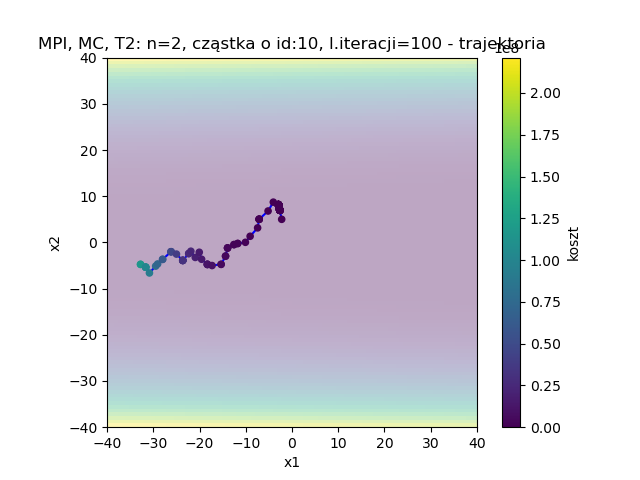
\includegraphics[width=1\linewidth]{grafiki/MPI_MC_T2/MPI_ MC_T2_trajectory_id10.png}
  \captionof{figure}{Trajektoria wybranej cząstki dla algorytmu MC dla zadania $2$.}
  \label{fig:trajektoriaWybrana:MC2}
\end{minipage}
\end{figure}

Na wykresach  \ref{fig:trajektoriaWybrana:MC1} - \ref{fig:trajektoriaWybrana:MC2} przedstawiono liczbę iteracji wykonaną w różnych procesach. Różnice w liczbie iteracji wykonanych w każdym z procesów wynikają z tego, że procesy te nie startują jednocześnie, ponieważ mają opóźnienia spowodowane koniecznością komunikacji.

% Liczba iteracji dla każdego z procesów

\begin{figure}[H]
\centering
\begin{minipage}[b]{\dimexpr.5\textwidth-1em}
  \centering
  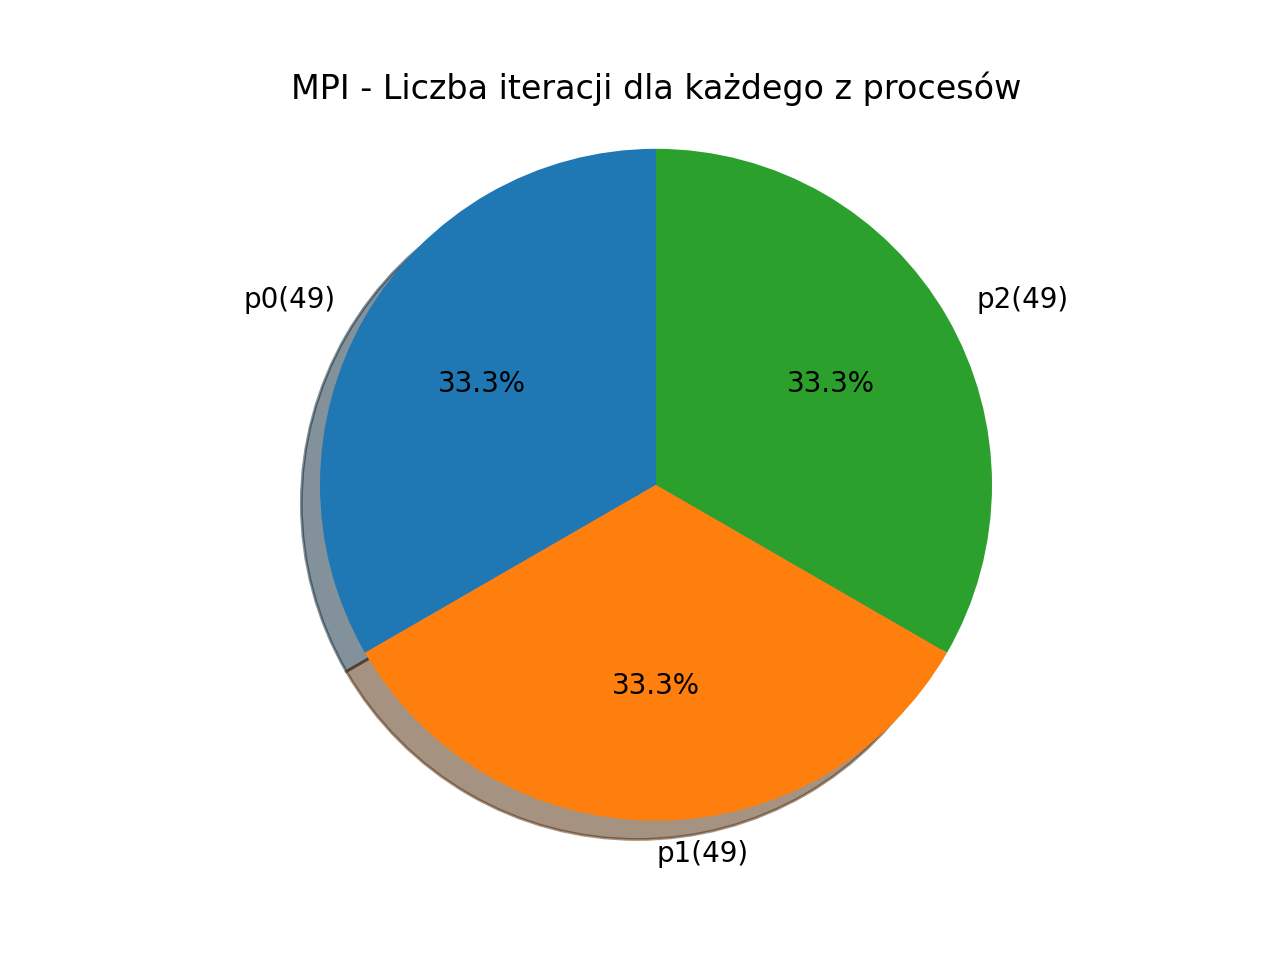
\includegraphics[width=1\linewidth]{grafiki/MPI_PSO_T1/MPI_PSO_T1_procIter.png}
  \captionof{figure}{Liczba iteracji dla każdego z procesów dla algorytmu PSO dla zadania $1$.}
  \label{fig:trajektoriaWybrana:PSO1}
\end{minipage} \hfill
\begin{minipage}[b]{\dimexpr.5\textwidth-1em}
  \centering
  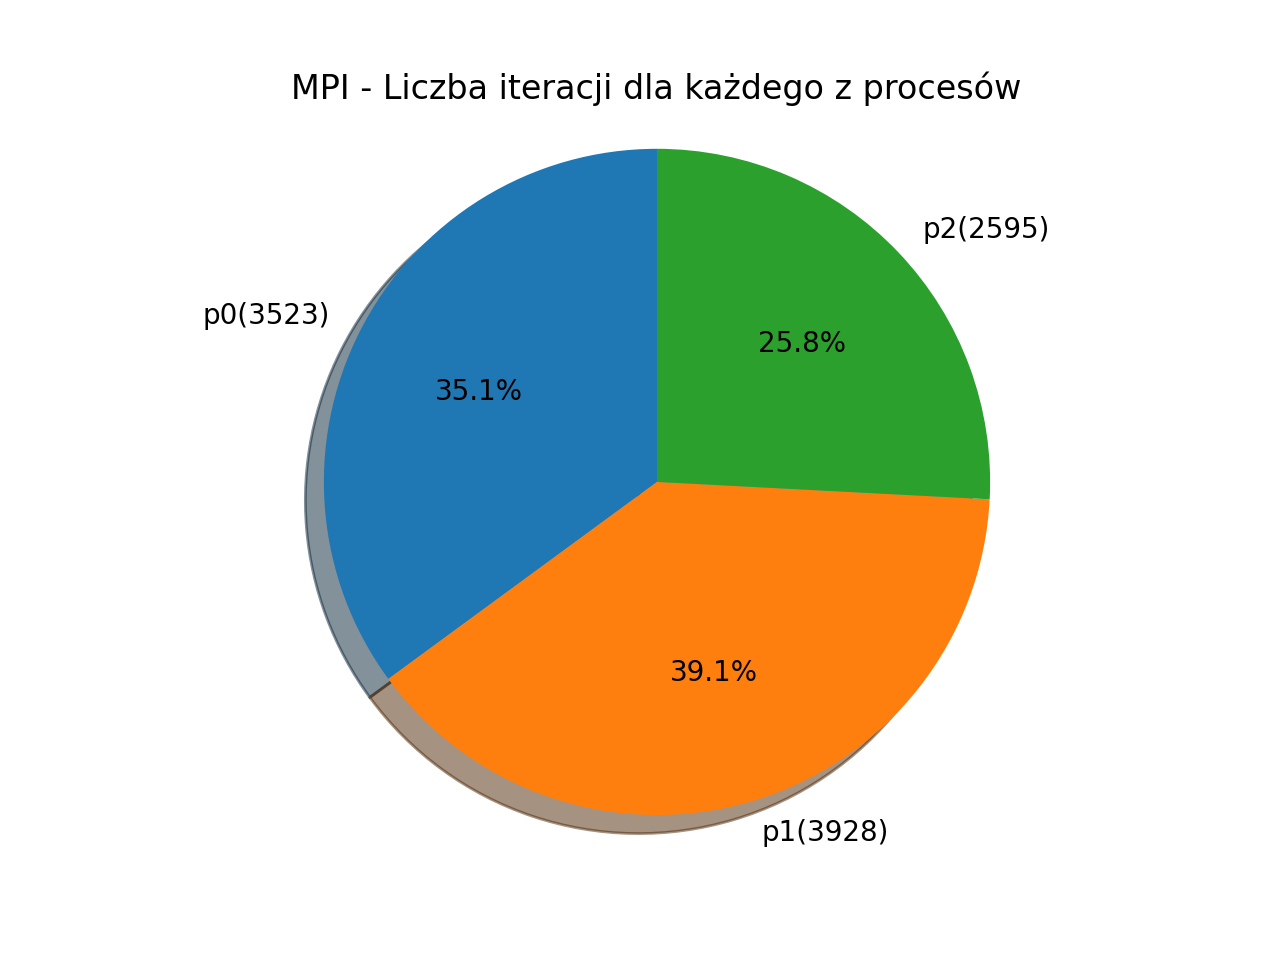
\includegraphics[width=1\linewidth]{grafiki/MPI_MC_T1/MPI_MC_T1_procIter.png}
  \captionof{figure}{Liczba iteracji dla każdego z procesów dla algorytmu MC dla zadania $1$.}
  \label{fig:trajektoriaWybrana:MC1}
\end{minipage}
\end{figure}

\begin{figure}[H]
\centering
\begin{minipage}[b]{\dimexpr.5\textwidth-1em}
  \centering
  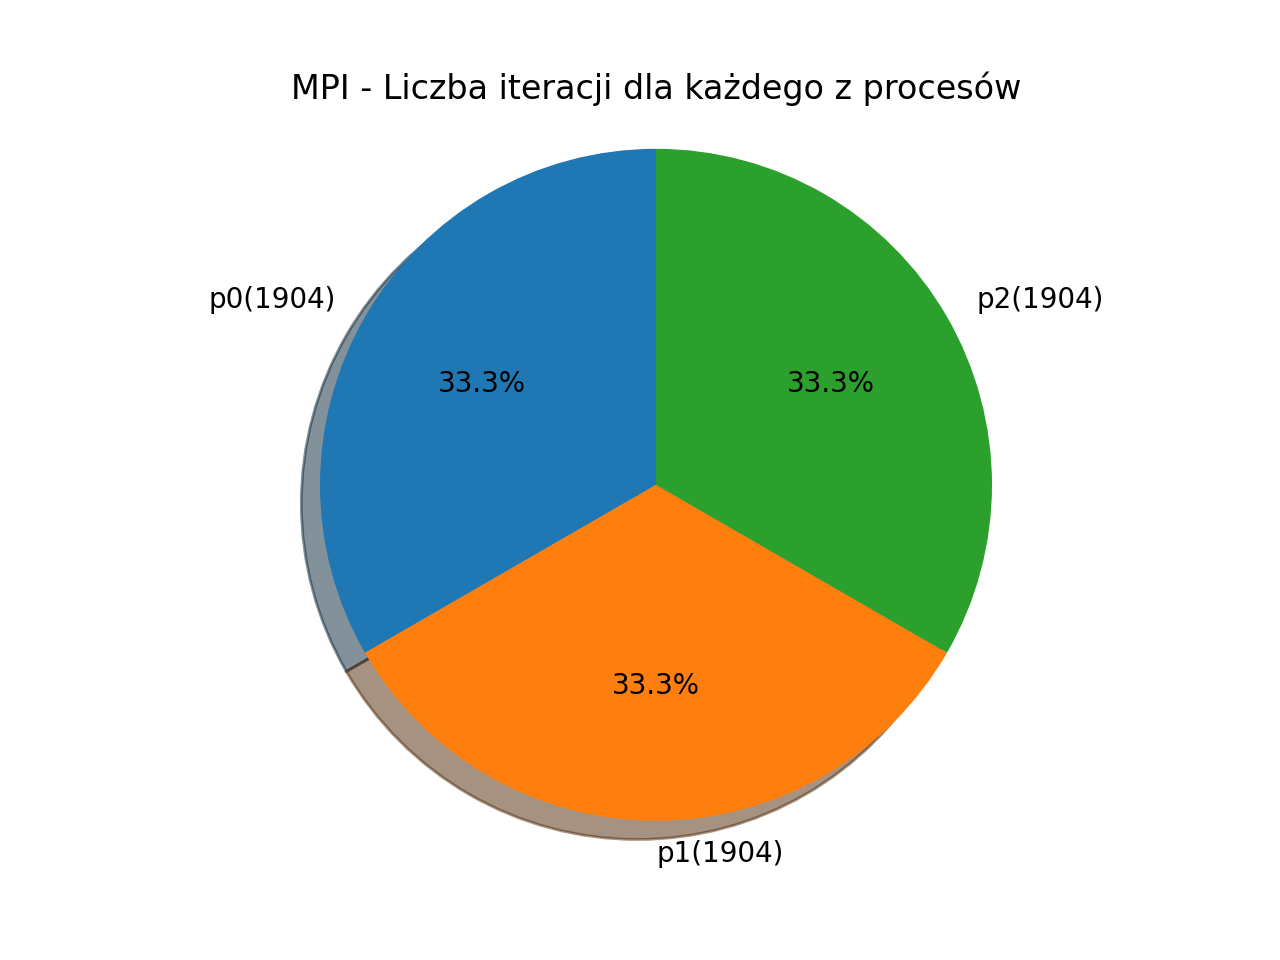
\includegraphics[width=1\linewidth]{grafiki/MPI_PSO_T2/MPI_PSO_T2_procIter.png}
  \captionof{figure}{Liczba iteracji dla każdego z procesów dla algorytmu PSO dla zadania $2$.}
  \label{fig:trajektoriaWybrana:PSO2}
\end{minipage} \hfill
\begin{minipage}[b]{\dimexpr.5\textwidth-1em}
  \centering
  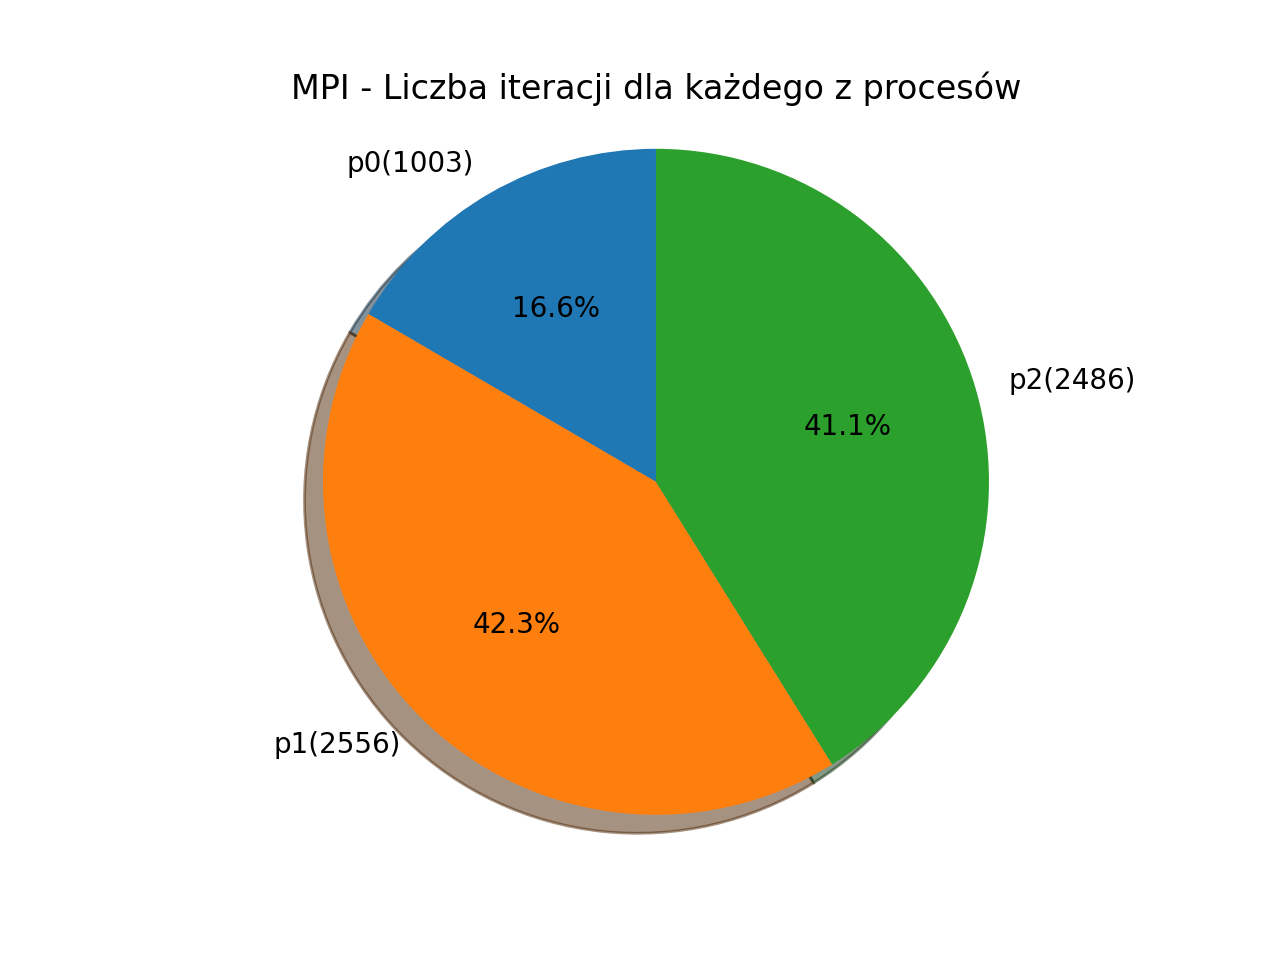
\includegraphics[width=1\linewidth]{grafiki/MPI_MC_T2/MPI_MC_T2_procIter.png}
  \captionof{figure}{Liczba iteracji dla każdego z procesów dla algorytmu MC dla zadania $2$.}
  \label{fig:trajektoriaWybrana:MC2}
\end{minipage}
\end{figure}



\subsection{Porównanie kosztu w CUDA} \label{sec:CUDA2}

Na wykresach \ref{fig:koszt:PSO1CUDAlog}-\label{fig:koszt:MC2CUDAlog} przedstawiono koszt dla obu zadań dla obu algorytmów. Dodatkowo koszt ten narysowano w skali logarytmicznej na wykresach \ref{fig:koszt:MC1CUDAlog}, \ref{fig:koszt:MC1CUDAlog}, \ref{fig:koszt:PSO2CUDAlog} i \ref{fig:koszt:MC2CUDAlog}.

%Funkcja kosztu - zad1 i zad2
\begin{figure}[H]
\centering
\begin{minipage}[b]{\dimexpr.5\textwidth-1em}
  \centering
  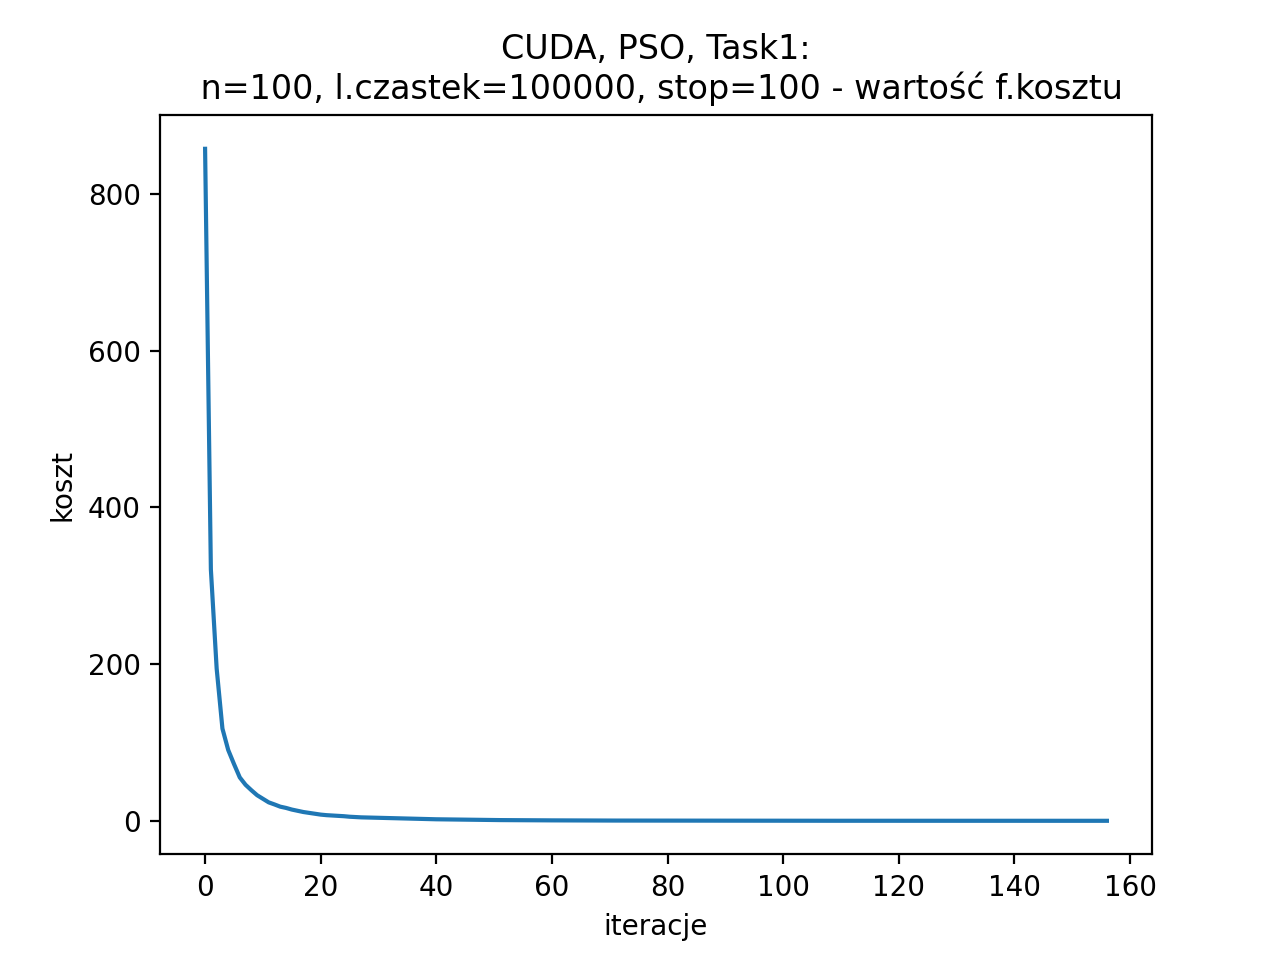
\includegraphics[width=1\linewidth]{grafiki/CUDA/CUDA_PSO_Task1_koszt_linear.png}
  \captionof{figure}{Wartość funkcji kosztu dla zadania $1$ dla algorytmu PSO.}
  \label{fig:koszt:PSO1CUDA}
\end{minipage} \hfill
\begin{minipage}[b]{\dimexpr.5\textwidth-1em}
  \centering
  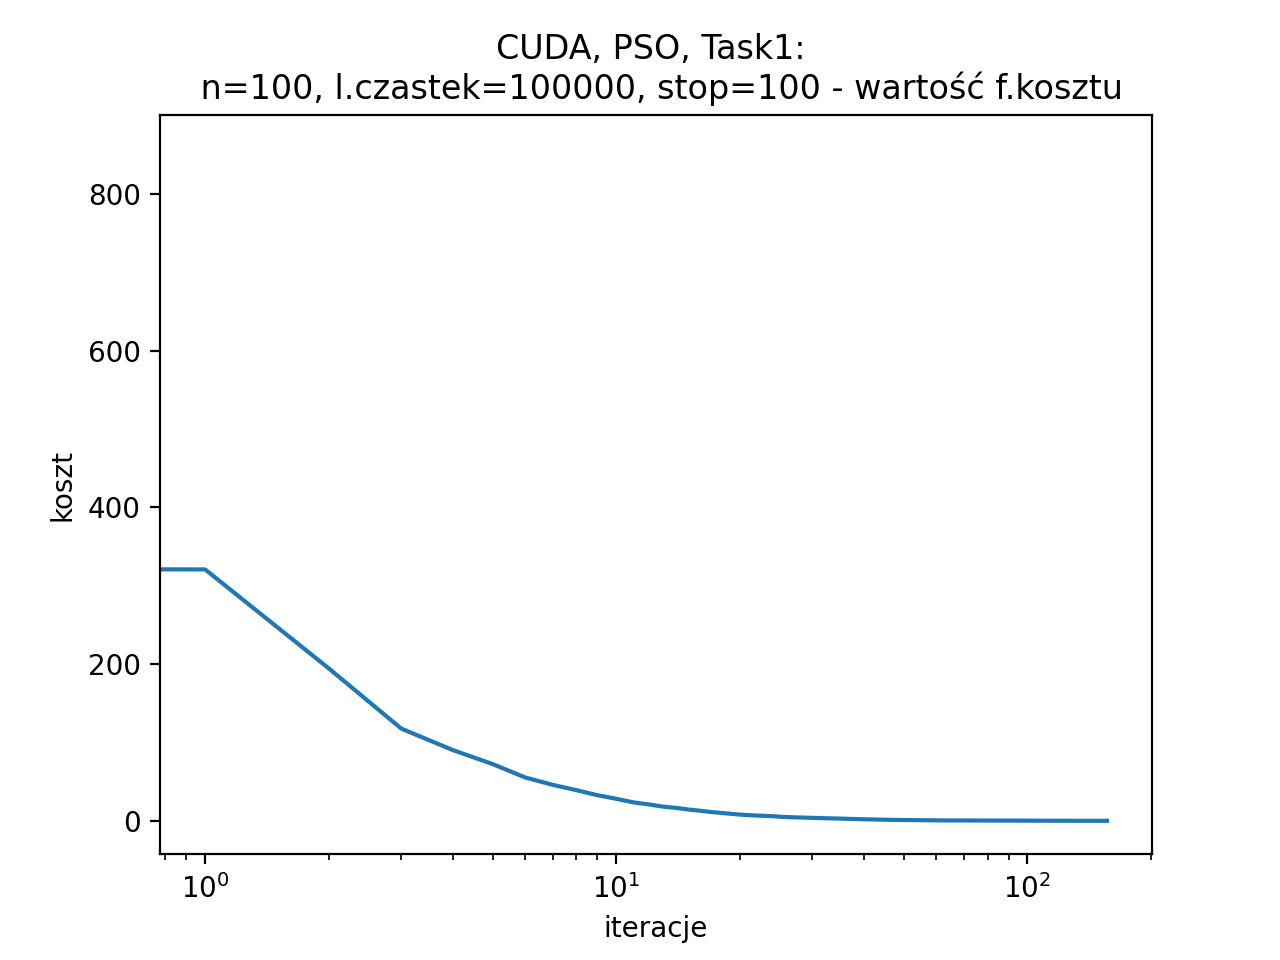
\includegraphics[width=1\linewidth]{grafiki/CUDA/CUDA_PSO_Task1_koszt_log.png}
  \captionof{figure}{Wartość funkcji kosztu w skali logarytmicznej dla zadania $1$ dla algorytmu PSO}
  \label{fig:koszt:PSO1CUDAlog}
\end{minipage}
\end{figure}

\begin{figure}[H]
\centering
\begin{minipage}[b]{\dimexpr.5\textwidth-1em}
  \centering
  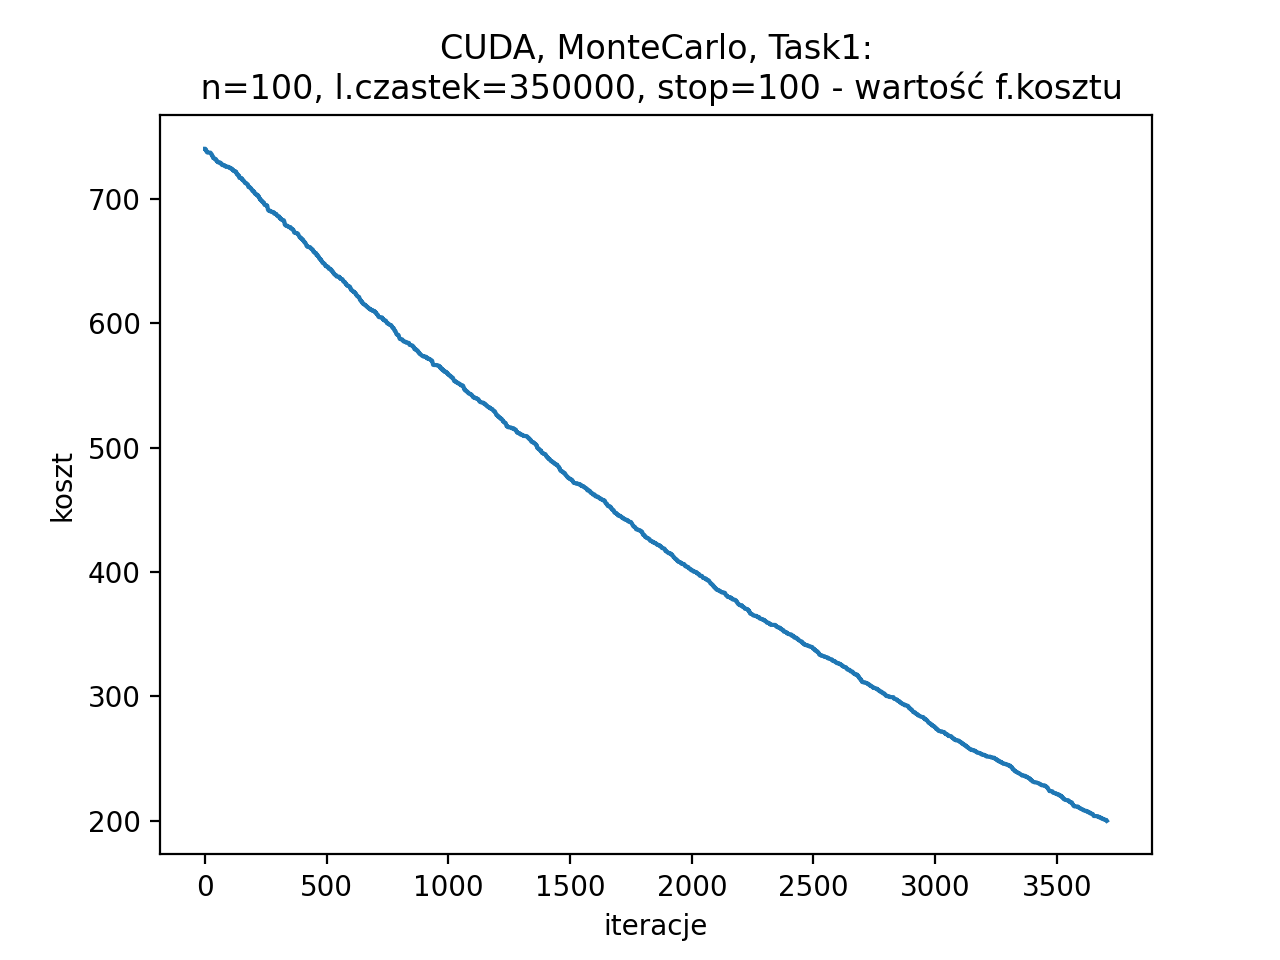
\includegraphics[width=1\linewidth]{grafiki/CUDA/CUDA_MonteCarlo_Task1_koszt_linear.png}
  \captionof{figure}{Wartość funkcji kosztu dla zadania $1$ dla algorytmu Monte Carlo.}
  \label{fig:koszt:PMC1CUDA}
\end{minipage} \hfill
\begin{minipage}[b]{\dimexpr.5\textwidth-1em}
  \centering
  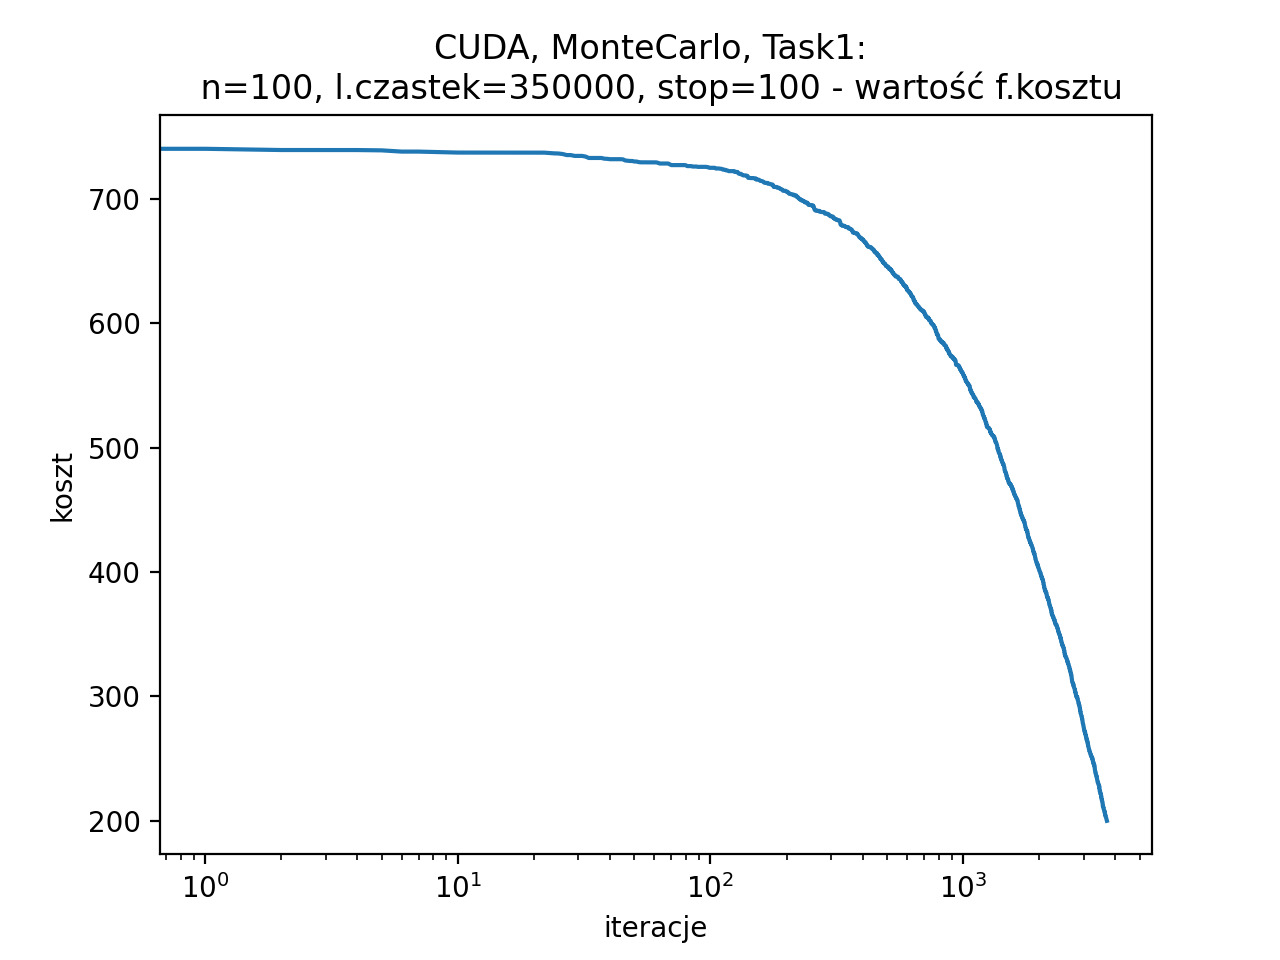
\includegraphics[width=1\linewidth]{grafiki/CUDA/CUDA_MonteCarlo_Task1_koszt_log.png}
  \captionof{figure}{Wartość funkcji kosztu w skali logarytmicznej dla zadania $1$ dla algorytmu Monte Carlo}
  \label{fig:koszt:MC1CUDAlog}
\end{minipage}
\end{figure}

\begin{figure}[H]
\centering
\begin{minipage}[b]{\dimexpr.5\textwidth-1em}
  \centering
  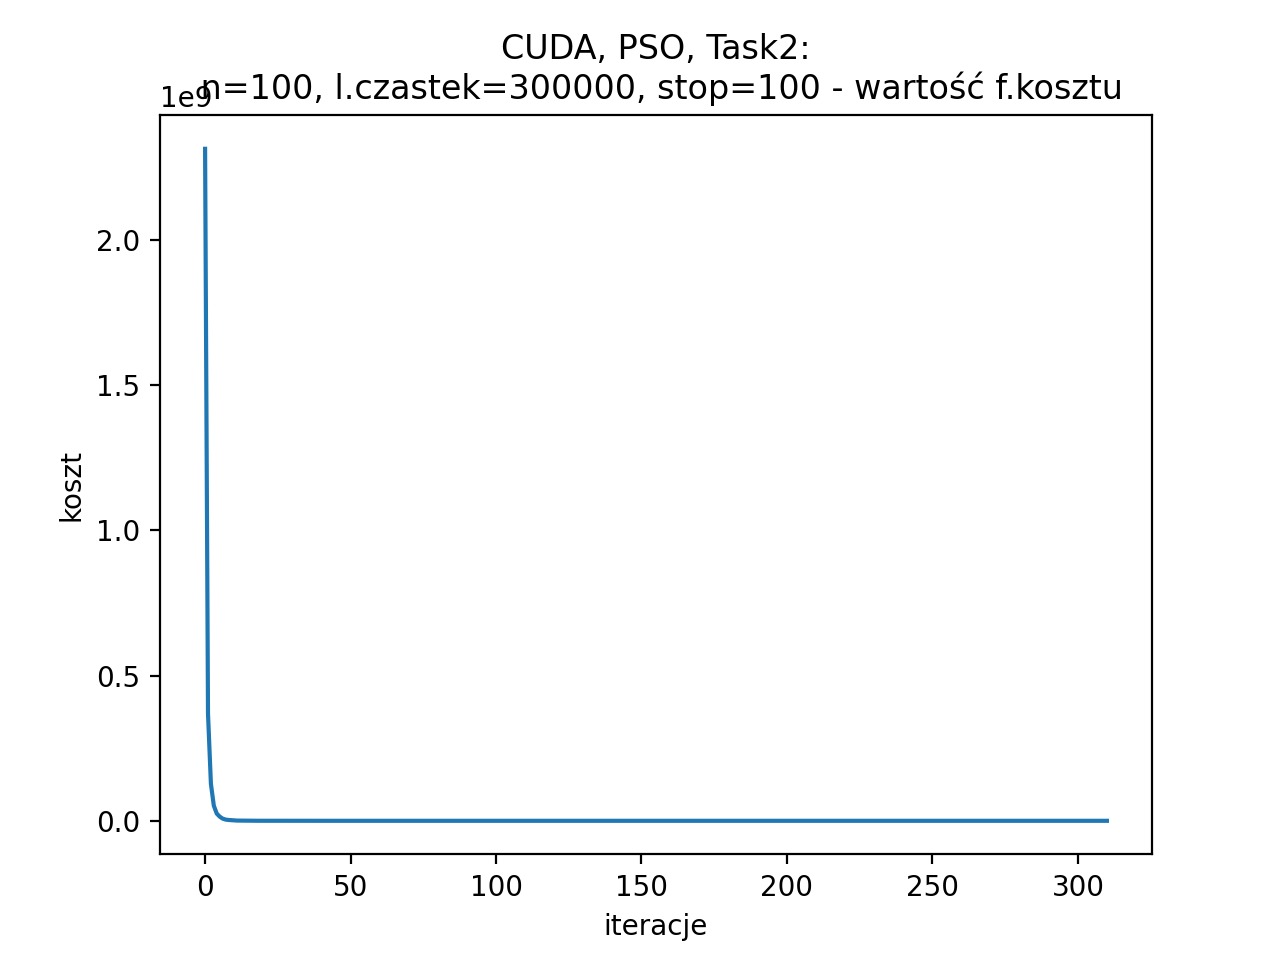
\includegraphics[width=1\linewidth]{grafiki/CUDA/CUDA_PSO_Task2_koszt_linear.png}
  \captionof{figure}{Wartość funkcji kosztu dla zadania $2$ dla algorytmu PSO.}
  \label{fig:koszt:PSO2CUDA}
\end{minipage} \hfill
\begin{minipage}[b]{\dimexpr.5\textwidth-1em}
  \centering
  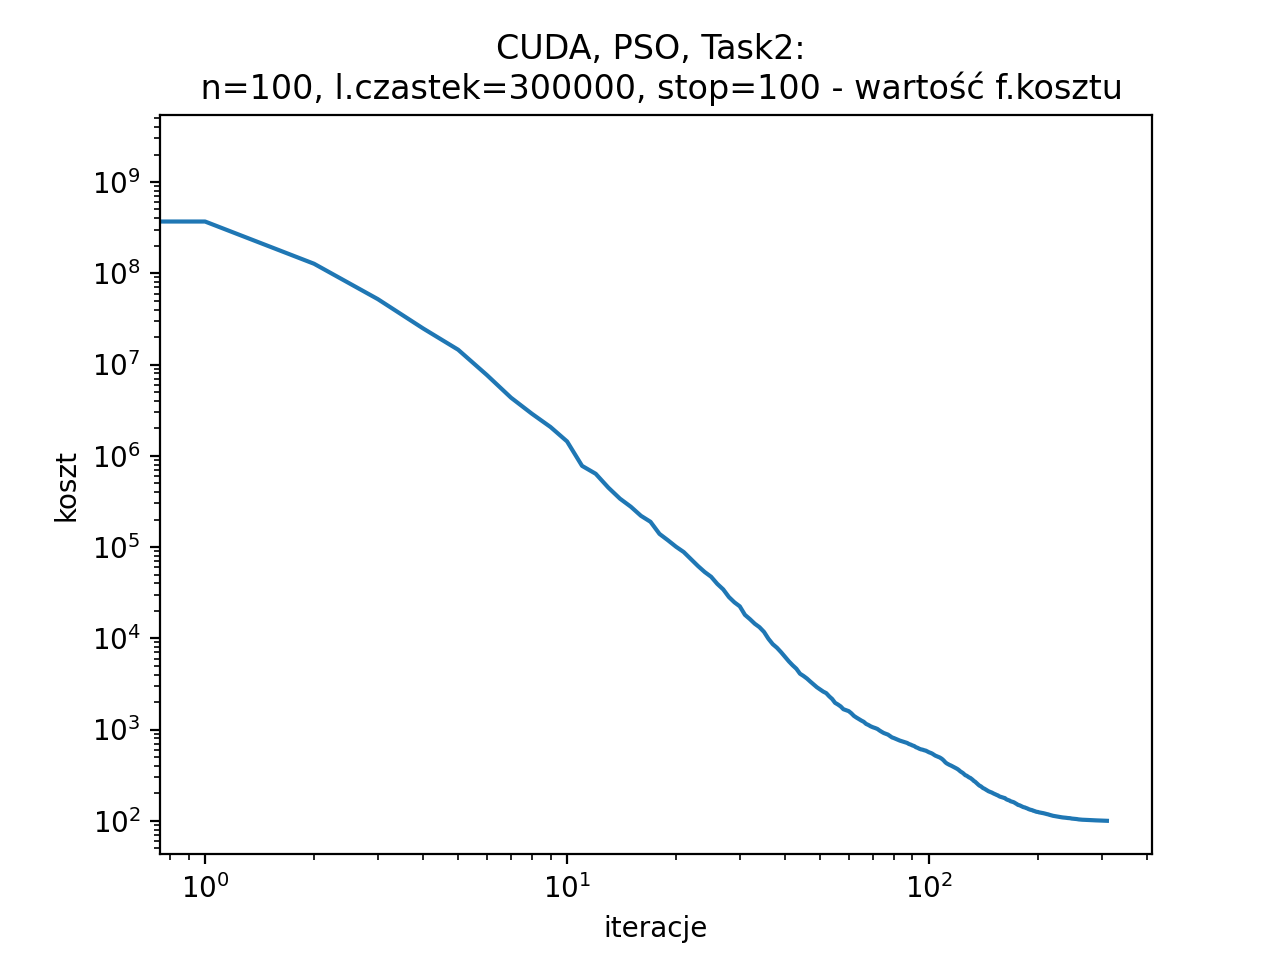
\includegraphics[width=1\linewidth]{grafiki/CUDA/CUDA_PSO_Task2_koszt_log.png}
  \captionof{figure}{Wartość funkcji kosztu w skali logarytmicznej dla zadania $2$ dla algorytmu PSO.}
  \label{fig:koszt:PSO2CUDAlog}
\end{minipage}
\end{figure}

\begin{figure}[H]
\centering
\begin{minipage}[b]{\dimexpr.5\textwidth-1em}
  \centering
  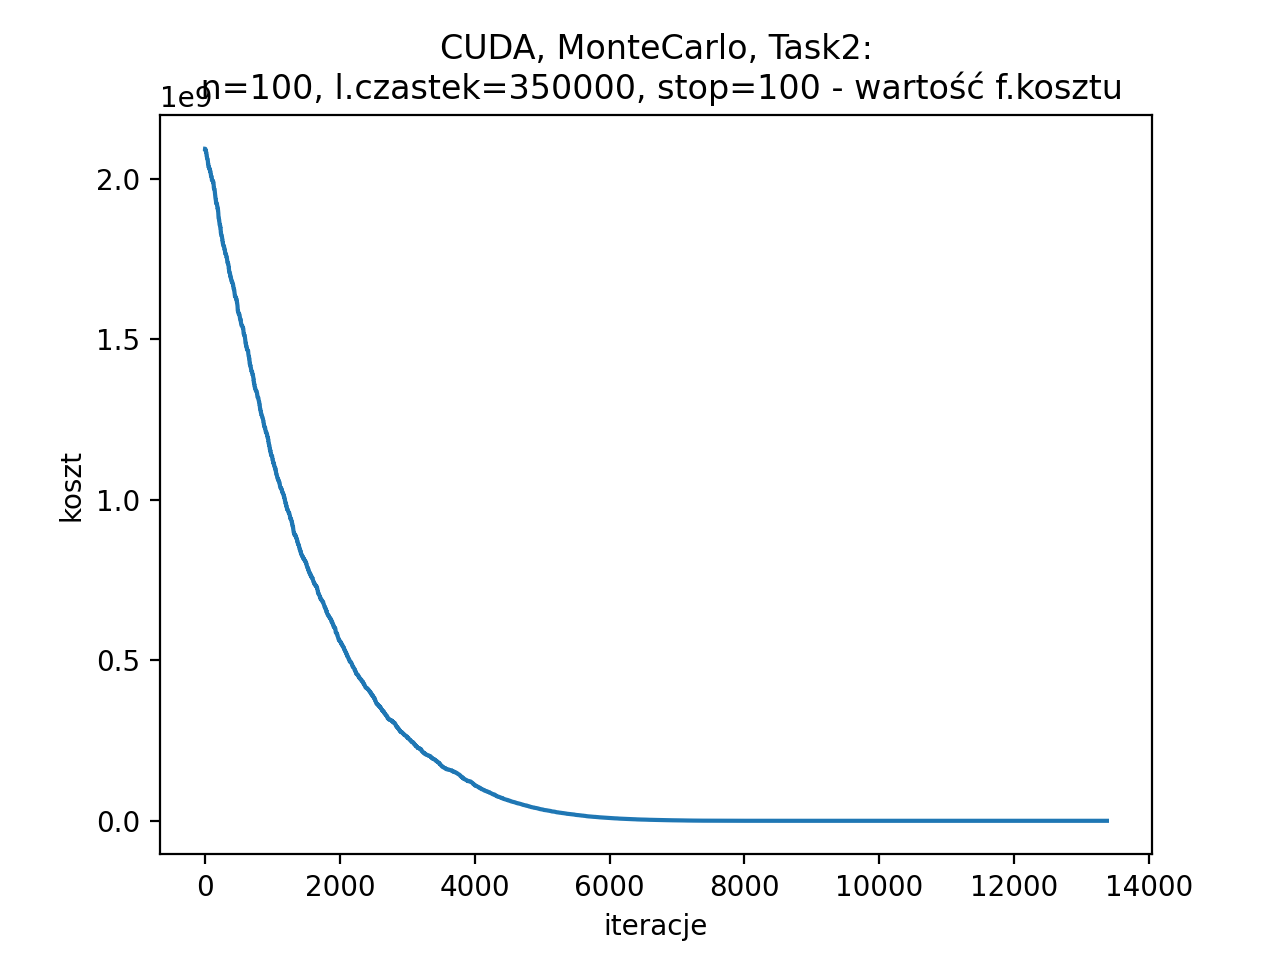
\includegraphics[width=1\linewidth]{grafiki/CUDA/CUDA_MonteCarlo_Task2_koszt_linear.png}
  \captionof{figure}{Wartość funkcji kosztu dla zadania $2$ dla algorytmu Monte Carlo.}
  \label{fig:koszt:MC2CUDA}
\end{minipage} \hfill
\begin{minipage}[b]{\dimexpr.5\textwidth-1em}
  \centering
  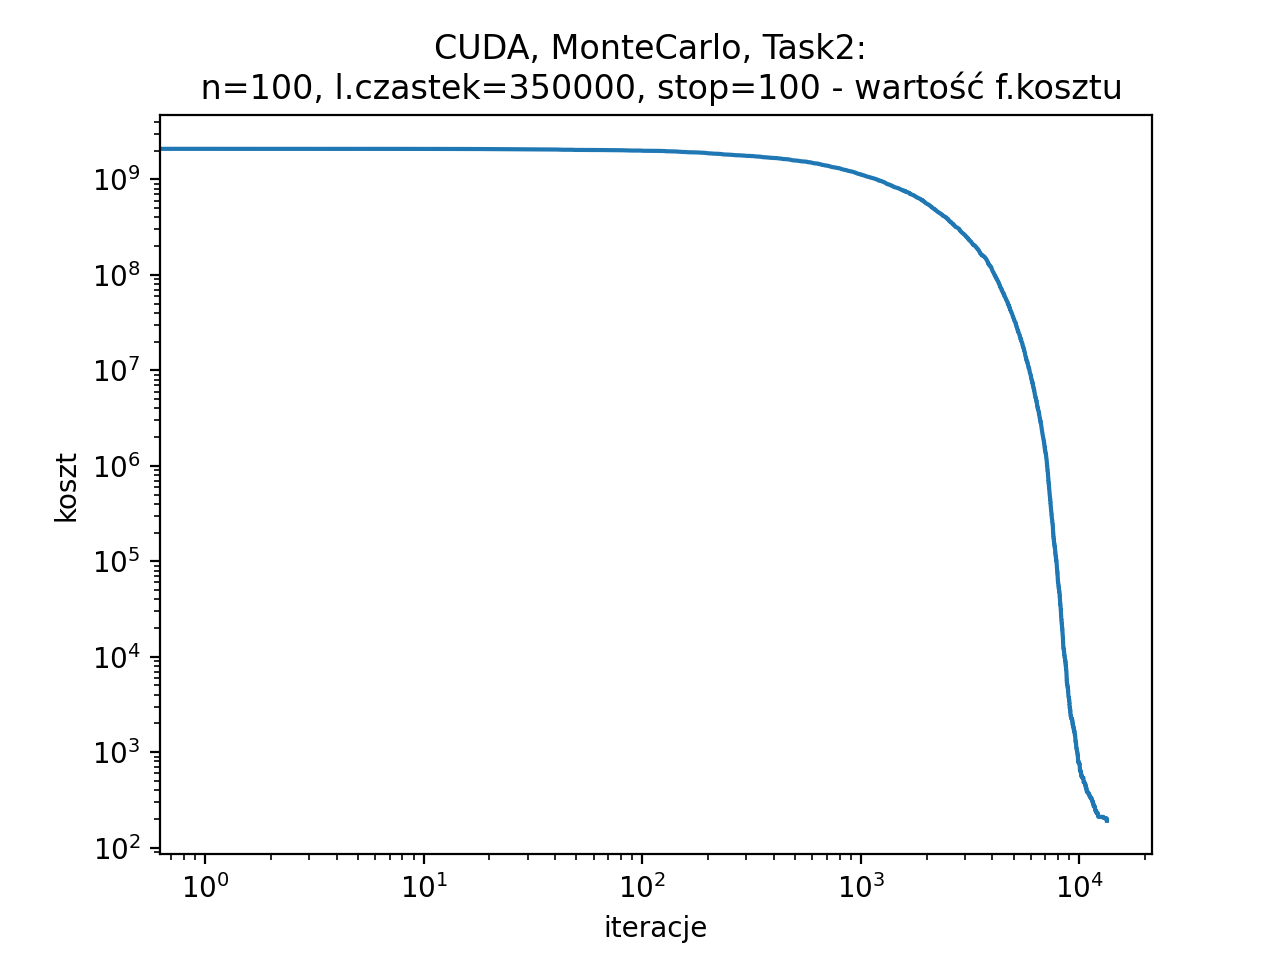
\includegraphics[width=1\linewidth]{grafiki/CUDA/CUDA_MonteCarlo_Task2_koszt_log.png}
  \captionof{figure}{Wartość funkcji kosztu w skali logarytmicznej dla zadania $2$ dla algorytmu Monte Carlo.}
  \label{fig:koszt:MC2CUDAlog}
\end{minipage}
\end{figure}

\section{Wnioski} 

Z wykresów \ref{fig:przysp:zad1}. i \ref{fig:przysp:zad2} widać, że przyspieszenie algorytmu PSO jest znacznie mniejsze niż przyspieszenie Monte Carlo. Prawdopodobnie wynika to z faktu, iż w implementacji PSO dużo czasu poświęcane jest komunikacji międzyprocesowej - w każdej iteracji procesy muszą sprawdzić czy znana jest nowa globalna najlepsza wartość. Metoda Monte Carlo nie używa komunikacji w trakcie obliczeń - wiadomości wysyłane są jedynie po znalezieniu zadowalającego rozwiązania przez jeden z procesów.

Warto także zwrócić uwagę, że niskie przyspieszenie PSO może także wynikać z względnie małej liczby cząstek. Do rozwiązania zadania $2$. dla $n \ = \ 20$ wymiarów użyto $10^{4}$ cząsteczek - znacznie więcej niż w pozostałych przypadkach. Ilość danych do przetworzenia związana z liczbą cząsteczek spowodowała rozmycie udziału komunikacji i w efekcie doprowadziła do większego przyspieszenia.

Kolejnym wnioskiem z przeprowadzonych badań jest to, że zmodyfikowany algorytm Monte Carlo prowadzi cząsteczkę prosto do najmniejszego kosztu bez "skakania" po całej przestrzeni kosztu, co powinno się dziać, jeśli zastosowalibyśmy czysty algorytm Monte Carlo. To powoduje niemożność wyjścia z lokalnych minimów. Ale ten problem jest rozwiązany dostatecznie dużą liczbą cząsteczek.

W równoległych procesach w MPI każdy proces zdąża zrobić różną liczbę iteracji z powodu opóźnień związanych z komunikacją (wykresy \ref{fig:trajektoriaWybrana:MC1} - \ref{fig:trajektoriaWybrana:MC2}).

Przy obliczeniach w CUDA zdecydowanie szybciej wyznacza się cząsteczkę spełniającą warunek stopu dla algorytmu PSO niż dla algorytmu Monte Carlo.
\end{document}







